\documentclass[12pt, a4paper]{article}

% ── Packages ──────────────────────────────────────────────────────────────────
\usepackage[T1]{fontenc}
\usepackage[utf8]{inputenc}
\usepackage[english]{babel}
\usepackage{lmodern}
\usepackage{microtype}
\usepackage{textcomp}
\usepackage{newunicodechar}
\newunicodechar{−}{-}
\usepackage{tikz}
\usetikzlibrary{positioning, arrows.meta, shapes.geometric, matrix,
                backgrounds, fit, calc,
                decorations.pathreplacing, decorations.markings}
\usepackage{geometry}
\usepackage{pgfplots}
\pgfplotsset{compat=1.18}
\usepackage{xcolor}
\usepackage{pgfplots}
\usepackage{pgfplotstable}
\usepackage{booktabs}
\usepackage{listings}
\usepackage{amsmath}
\usepackage{pgfplots}
\usepackage{pgfplotstable}
\pgfplotsset{compat=1.18}
\definecolor{cgray}{RGB}{136,135,128}
\graphicspath{{Images/}}

\usepackage{tikz}
\usetikzlibrary{arrows.meta}
\usepackage{pgfplots}
\pgfplotsset{compat=1.18}
\usepackage{booktabs}
\usepackage{float}
\usepackage{amsmath}

\definecolor{col-teal}  {RGB}{29,158,117}
\definecolor{col-blue}  {RGB}{55,138,221}
\definecolor{col-coral} {RGB}{216,90,48}
\definecolor{col-purple}{RGB}{127,119,221}

\pgfplotsset{
  approxstyle/.style={
    width=0.95\linewidth,
    height=4.8cm,
    axis lines=left,
    grid=major,
    grid style={dotted,gray!35},
    tick label style={font=\footnotesize},
    label style={font=\small},
    title style={font=\small\bfseries},
    xmin=0, xmax=6.30,
    ymin=-1, ymax=21,
    xtick={0,1.5708,3.1416,4.7124,6.2832},
    xticklabels={$0$,$\frac{\pi}{2}$,$\pi$,$\frac{3\pi}{2}$,$2\pi$},
    xlabel={$x_1$},
    legend style={
      font=\footnotesize,
      at={(0.02,0.98)},
      anchor=north west,
      draw=gray!40,
      fill=white,
      fill opacity=0.85,
      text opacity=1
    },
    clip=false
  }
}
% ── shared style ──────────────────────────────────────────────────
\pgfplotsset{
  tut/.style={
    width=0.92\linewidth,
    height=5.5cm,
    axis lines=left,
    grid=major,
    grid style={dotted, gray!40},
    tick label style={font=\footnotesize},
    label style={font=\small},
    title style={font=\small\bfseries},
    legend style={font=\footnotesize, at={(0.98,0.98)},
                  anchor=north east, draw=gray!40},
    clip=false,
  }
}
\lstset{
  language=Python,
  basicstyle=\ttfamily\small,
  keywordstyle=\color{blue}\bfseries,
  commentstyle=\color{gray}\itshape,
  stringstyle=\color{teal},
  numbers=left,
  numberstyle=\tiny\color{gray},
  backgroundcolor=\color{gray!10},
  breaklines=true,
  frame=single,
  showstringspaces=false
}
\usepackage{setspace}
\setstretch{1.25}
\usepackage{parskip}
\setlength{\parskip}{6pt}
\usepackage{amsmath, amssymb, bm}
\usepackage{booktabs}
\usepackage{array}
\usepackage{tabularx}
\usepackage{longtable}
\usepackage{float}
\usepackage{ragged2e}
\usepackage{enumitem}
\usepackage{graphicx}
\graphicspath{{Pics/}}

\definecolor{cblue}{RGB}{56,138,221}
\definecolor{cpurple}{RGB}{127,119,221}
\definecolor{camber}{RGB}{186,117,23}
\definecolor{cteal}{RGB}{29,158,117}
\definecolor{ccoral}{RGB}{216,90,48}
\definecolor{accentblue}{RGB}{0,114,206}
\usepackage[
  colorlinks=true,
  linkcolor=accentblue,
  citecolor=accentblue,
  urlcolor=accentblue
]{hyperref}
\usepackage{cleveref}
\usepackage{natbib}
\bibliographystyle{plainnat}

\title{PINNs Tutorial}
\author{Ahmad Azzeh}
\date{May 2026}

\begin{document}

\maketitle
\tableofcontents
\newpage




\section{Introduction of physics informed neural networks  "PINNs" }


This body of work is made as a tutorial/thesis to explain PINNs and their application to my current idea of \textit{temporal thermal field reconstruction from spare sensors using PINNs in Smart Metal Alloys}. 

The discussion will start with the basics of neural networks and the math behind it, then moving on to PINNs, their application, types,... etc. Finally, ending with a PINN model for the said problem.



\subsection{PINN vs NN}

% add definition of neural networks and PINNs 

Neural networks and Physics Informed Neural Networks are two vastly different things. Although they similiar in structure, they differ in principle. It would ridiclious to feed a normal neural network data that is of high dimensions and expect it to map out the non-linear behaviour of the function. However, introducing a factor that regulates the activity of the neural network, the factor could be known imperical data or governing laws that are known, to produce a well behaved output. This design allows for a better stearing of the network into the correct answer even if only few data points are available \citep{raissi2019}.



\subsection{The issue at hand}

\subsection{PINN vs FEM/FVM}

\subsection{Mathematical model of the equation}
% ══════════════════════════════════════════════════════════════════════════════
\section{The Perceptron — One Neuron, One Decision}
\label{sec:perceptron}
% ──────────────────────────────────────────────────────────────────────────────

The \textbf{perceptron} is the fundamental building block of every neural network.
It is a single artificial neuron that takes a set of numerical inputs, weighs each
one according to its importance, sums the result, and passes it through an
\textbf{activation function} to produce an output. Before understanding how layers
of neurons work together, it is necessary to understand what one neuron does on
its own.\citep{rosenblatt1958}

\subsection{What a Perceptron Does}

A perceptron with $n$ inputs $x_1, x_2, \ldots, x_n$ computes:

\begin{equation}
    z = w_1 x_1 + w_2 x_2 + \cdots + w_n x_n + b
      = \sum_{i=1}^{n} w_i x_i + b
    \label{eq:perceptron_preact}
\end{equation}

\begin{equation}
    a = \sigma(z)
    \label{eq:perceptron_act}
\end{equation}



Where $b$ is the bais term that adjusts the perceptron so it knows when to activate and is independndant of any input. The bais shifts the line of the equation either up, down, left or right.

\begin{figure} [H]
    \centering
    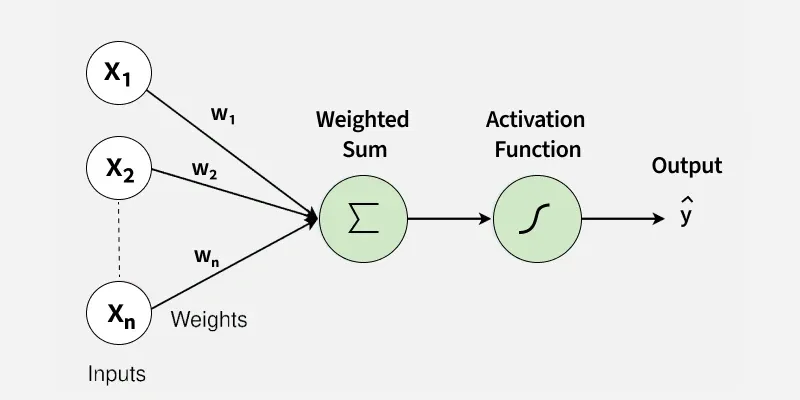
\includegraphics[width=1\linewidth]{image.png}
    \caption{Simple model of a perceptron}
    \label{fig:Perceptron model}
\end{figure}

Each weight $w_i$ controls how much input $x_i$ influences the result, this is also ture for the value of $x_i$. For example if $x_1$ is a large value where $w_1$ is much greater than $w_2$, the large
$w_1$ means that the $w_1x_i$ will influence the result much more than $w_2x_2$. A value near zero
means the perceptron will ignores it. 




The sum of each input with its respective weight is called \emph{the weighted sum}. This is then passed onto something called an \emph{activation function} these introduce the non-linearity needed for us to approximate our complex functions. 

\subsection{Activation Functions}

Activation functions are still an on going topic where new techniques and mixes are being used to find  the best combination, however for our needs we only need to talk about three activation functions:

\begin{itemize}
    \item \textbf{ReLU}: $\sigma(z) = \max(0, z)$. Computationally cheap but
    non-differentiable at $z = 0$. \citep{nair2010}

    \item \textbf{Sigmoid}: $\sigma(z) = 1/(1 + e^{-z})$. Smooth and bounded
    in $(0,1)$, but suffers from vanishing gradients in deep networks.\citep{lecun1998}

    \item \textbf{Tanh}: $\sigma(z) = \tanh(z)$. Smooth, bounded in $(-1,1)$,
    zero-centred, and infinitely differentiable. \citep{lecun1998}
\end{itemize}
\begin{figure}[H]
\centering

% ── ReLU ──────────────────────────────────────────────────────────────────────
\begin{minipage}[t]{0.32\textwidth}
    \centering
    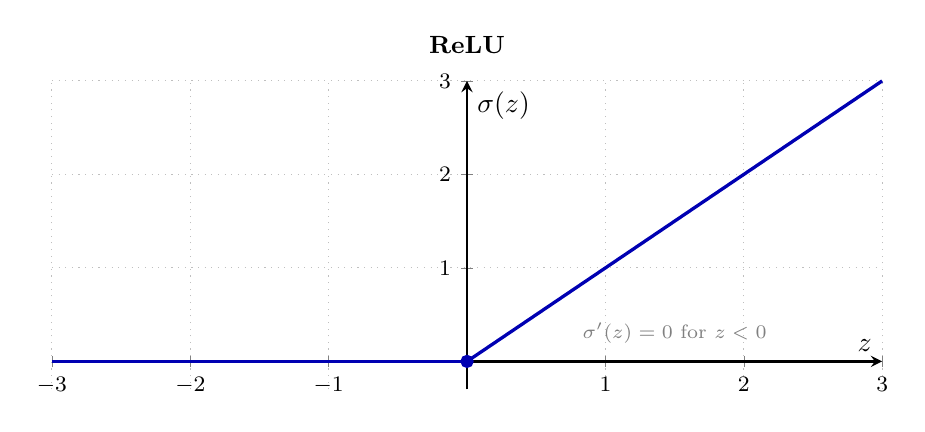
\begin{tikzpicture}
        \begin{axis}[
            width=\linewidth,
            height=5.5cm,
            xlabel={$z$},
            ylabel={$\sigma(z)$},
            title={\textbf{ReLU}},
            title style={font=\small},
            label style={font=\small},
            tick label style={font=\footnotesize},
            xmin=-3, xmax=3,
            ymin=-0.3, ymax=3,
            xtick={-3,-2,-1,0,1,2,3},
            ytick={0,1,2,3},
            axis lines=center,
            axis line style={-stealth},
            grid=major,
            grid style={dotted, gray!50},
            samples=200,
            thick,
            clip=false,
        ]
        % ReLU: max(0,z)
        \addplot[blue!70!black, very thick, domain=-3:0] {0};
        \addplot[blue!70!black, very thick, domain=0:3]  {x};
        % non-differentiable kink marker
        \addplot[blue!70!black, only marks, mark=*, mark size=2pt]
            coordinates {(0,0)};
        % annotation
        \node[font=\scriptsize, align=center, text=gray]
            at (axis cs:1.5, 0.3)
            {$\sigma'(z)=0$ for $z<0$};
        \end{axis}
    \end{tikzpicture}
    \[\sigma(z) = \max(0,\,z)\]
\end{minipage}
\hfill
% ── Sigmoid ───────────────────────────────────────────────────────────────────
\begin{minipage}[t]{0.32\textwidth}
    \centering
    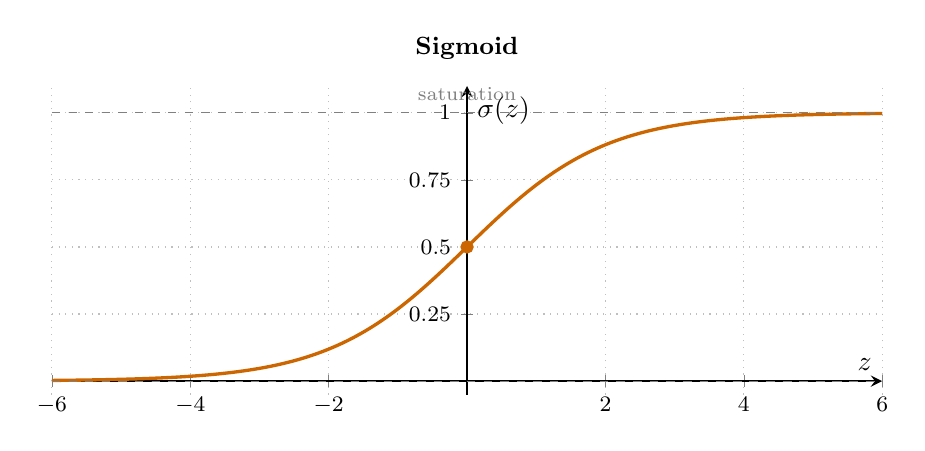
\begin{tikzpicture}
        \begin{axis}[
            width=\linewidth,
            height=5.5cm,
            xlabel={$z$},
            ylabel={$\sigma(z)$},
            title={\textbf{Sigmoid}},
            title style={font=\small},
            label style={font=\small},
            tick label style={font=\footnotesize},
            xmin=-6, xmax=6,
            ymin=-0.05, ymax=1.1,
            xtick={-6,-4,-2,0,2,4,6},
            ytick={0,0.25,0.5,0.75,1},
            yticklabels={$0$,$0.25$,$0.5$,$0.75$,$1$},
            axis lines=center,
            axis line style={-stealth},
            grid=major,
            grid style={dotted, gray!50},
            samples=300,
            thick,
            clip=false,
        ]
        \addplot[orange!80!black, very thick, domain=-6:6]
            {1/(1+exp(-x))};
        % saturation dashed lines
        \addplot[gray, dashed, thin, domain=-6:6] {1};
        \addplot[gray, dashed, thin, domain=-6:6] {0};
        % midpoint marker
        \addplot[orange!80!black, only marks, mark=*, mark size=2pt]
            coordinates {(0,0.5)};
        \node[font=\scriptsize, align=center, text=gray]
            at (axis cs:0, 1.07)
            {saturation};
        \end{axis}
    \end{tikzpicture}
    \[\sigma(z) = \dfrac{1}{1+e^{-z}}\]
\end{minipage}
\hfill
% ── Tanh ──────────────────────────────────────────────────────────────────────
\begin{minipage}[t]{0.32\textwidth}
    \centering
    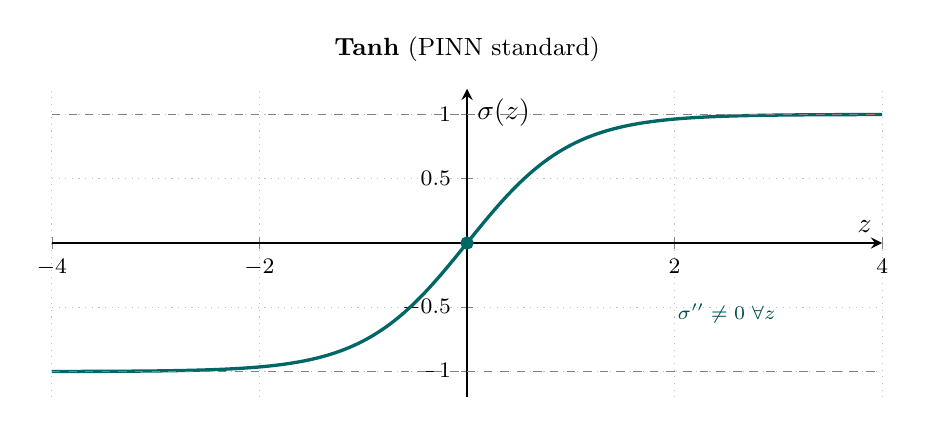
\begin{tikzpicture}
        \begin{axis}[
            width=\linewidth,
            height=5.5cm,
            xlabel={$z$},
            ylabel={$\sigma(z)$},
            title={\textbf{Tanh} {\small(PINN standard)}},
            title style={font=\small},
            label style={font=\small},
            tick label style={font=\footnotesize},
            xmin=-4, xmax=4,
            ymin=-1.2, ymax=1.2,
            xtick={-4,-2,0,2,4},
            ytick={-1,-0.5,0,0.5,1},
            axis lines=center,
            axis line style={-stealth},
            grid=major,
            grid style={dotted, gray!50},
            samples=300,
            thick,
            clip=false,
        ]
        \addplot[teal!80!black, very thick, domain=-4:4]
            {tanh(x)};
        % saturation dashed lines
        \addplot[gray, dashed, thin, domain=-4:4] {1};
        \addplot[gray, dashed, thin, domain=-4:4] {-1};
        % origin marker
        \addplot[teal!80!black, only marks, mark=*, mark size=2pt]
            coordinates {(0,0)};
        % second derivative annotation
        \node[font=\scriptsize, align=center, text=teal!60!black]
            at (axis cs:2.5, -0.55)
            {$\sigma'' \neq 0\;\forall z$};
        \end{axis}
    \end{tikzpicture}
    \[\sigma(z) = \tanh(z)\]
\end{minipage}

\caption{The three activation functions}
\label{fig:activation_functions}
\end{figure}

\subsection{what are activation functions and when are they used?}

\text Activation functions came to be to introduce nonlinearity to the data. Without this nonlinearity the data from the neural networks would just become linear transformers. In this tutorial we will focus on the basic activation functions. 

From the theory of approximation and based on empirical data, a mathematical model of the biological neuron activation was made and gave rise to the Sigmoid function and the Tanh function (hyperbolic).  

\subparagraph{ A bit of history }
the S-shaped of the sigmoid curve approximates a step function and outputs values in (0,1), making it ideal for probabilistic interpretations like binary classification. It was the default activation function in the 1980s and early 1990s. \citep{lecun1998}

Hyperbolic tangent (Tanh), outputs values in the range (−1,1), centering the activations around zero. This property accelerates convergence in the early layers of a network by providing stronger gradients compared to the sigmoid function. As a result, tanh became a popular choice of activation function during the late 1990s and early 2000s, especially for neural networks that required more robust training dynamics. This was due to its differentiability everywhere and centering around zero.


Even though the development of activation functions have made it possible to solve a lot of problems and they are indeed powerful tools. However, they come with their own limits. 
One cannot just simply apply the same activation function and hope for the best, one must consider if the chosen function applies to the problem at hand or must reach out for a different tool in the toolbox. 

\textbf{Sigmoid ($\sigma$) }
\begin{itemize}
    \item Domain: The domain of the sigmoid function is all real numbers.
    \item Asymptotes: As $x$ approaches positive infinity, $\sigma(x)$ approaches 1. Conversely, as $x$ approaches negative infinity, $\sigma(x)$ approaches 0. 
    \item Differentiability: The sigmoid function is differentiable, which allows for the calculation of gradients during the training of machine learning models.
\end{itemize}

\begin{figure}[H]
    \centering
    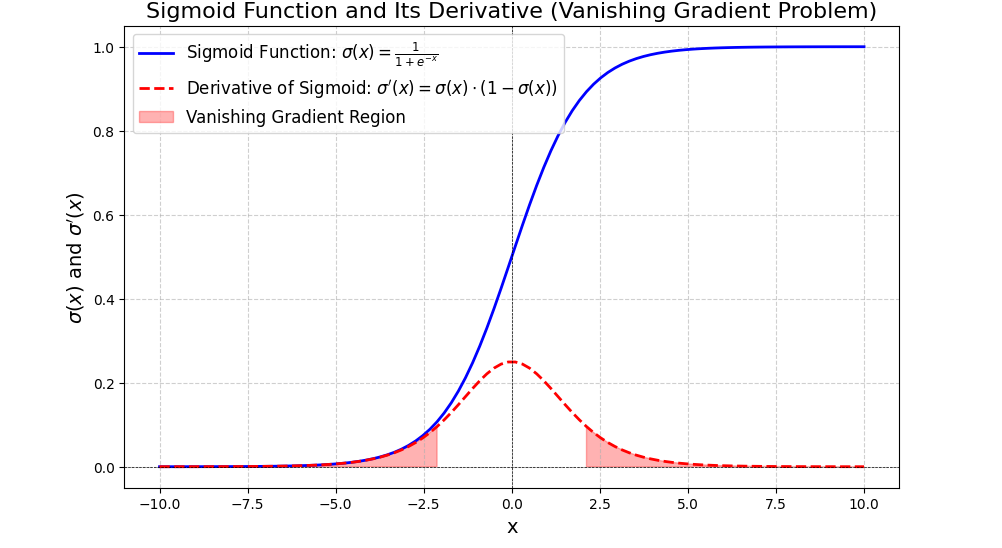
\includegraphics[width=0.75\linewidth]{Sigmoid function and gradient.png}
    \caption{ADD IN LATER}
    \label{fig:SIGMA grad}
\end{figure}
In backpropagation ( A process discussed in section \ref{sec:backprop_detail} we face an issue with this function, called the vanishing gradient\citep{bengio1994}.
In backpropagation the value of the gradient at the said point is used to adjust for the weights of the inputs. However, if the gradient value is too small, then the weight doesn't get adjusted correctly or stops being considered.
This can be better seen when drawing out the derivative function of the sigmoid as seen in \ref{fig:SIGMA grad}. \citep{bengio1994,hochreiter1991}


\textbf{Tanh}


Similar in shape to the Sigmoid function, however;
\begin{itemize}
    \item Centered around zero, why is this helpful in training will become more clearer in later sections.
    \item Improved convergence and gradient decent efficiency.
    \item Output between (-1,1).
\end{itemize}

Tanh deals better with the vanishing gradient problem, but still faces it with huge or very small value inputs. Thus, one must first normalize the data before introducing it to the network.\citep{lecun1998}
\begin{figure}[H]
    \centering
    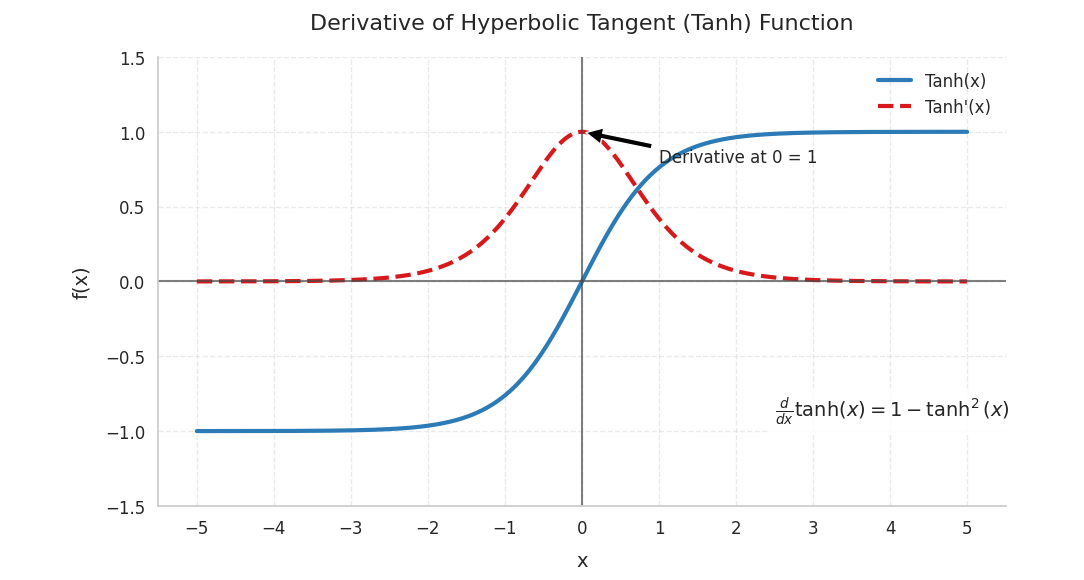
\includegraphics[width=0.75\linewidth]{Tanh grad.png}
    \caption{Enter Caption}
    \label{fig:Tanh grad}
\end{figure}

\textbf{RELU}
\begin{itemize}
    \item Allows positive values to pass unchanged and sets negative values to zero.
    \item Simple and computationally efficient activation function.
    \item Helps maintain non-linearity in neural networks.
    \item Reduces the vanishing gradient problem compared to older functions.
\end{itemize}
The simplicity of this function allows for much easier computation. However, this too has its own issues and variations, that sadly will not be discussed going forward as the focus is on PINNs. \citep{nair2010}










\subsection{The math behind it - A simple Intro}
\label{sec:intromath}

\begin{figure}[H]
\centering
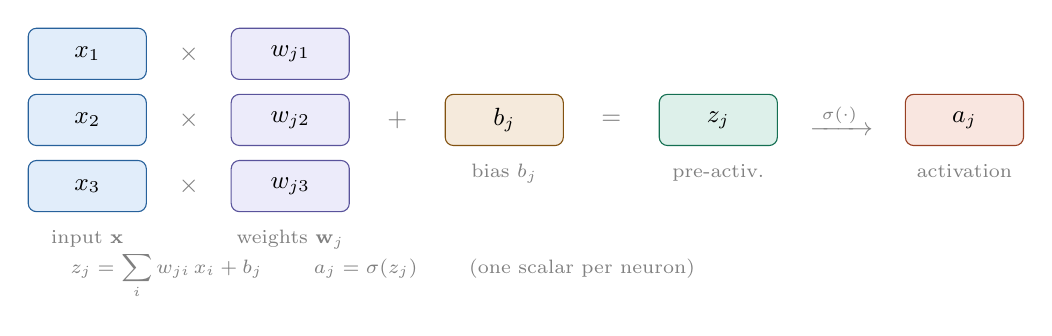
\begin{tikzpicture}[
  node distance=6pt and 14pt,
  every node/.style={font=\small},
  lbl/.style={font=\scriptsize, text=gray},
  cell/.style 2 args={
    draw=#1!70!black, fill=#1!15,
    rounded corners=3pt,
    minimum width=1.5cm, minimum height=0.65cm,
    inner sep=4pt, font=\small\bfseries, align=center
  }
]

% ── inputs ──────────────────────────────────────────
\node[cell={cblue}{}](x1){$x_1$};
\node[cell={cblue}{}, below=5pt of x1](x2){$x_2$};
\node[cell={cblue}{}, below=5pt of x2](x3){$x_3$};
\node[lbl, below=3pt of x3]{input $\mathbf{x}$};

% ── × signs ─────────────────────────────────────────
\node[text=gray, right=8pt of x1](m1){$\times$};
\node[text=gray, right=8pt of x2](m2){$\times$};
\node[text=gray, right=8pt of x3](m3){$\times$};

% ── weights ─────────────────────────────────────────
\node[cell={cpurple}{}, right=8pt of m1](w1){$w_{j1}$};
\node[cell={cpurple}{}, right=8pt of m2](w2){$w_{j2}$};
\node[cell={cpurple}{}, right=8pt of m3](w3){$w_{j3}$};
\node[lbl, below=3pt of w3]{weights $\mathbf{w}_j$};

% ── + bias ──────────────────────────────────────────
\node[text=gray, right=10pt of w2](plus){$+$};
\node[cell={camber}{}, right=10pt of plus](b){$b_j$};
\node[lbl, below=3pt of b]{bias $b_j$};

% ── = pre-activation ────────────────────────────────
\node[text=gray, right=10pt of b](eq){$=$};
\node[cell={cteal}{}, right=10pt of eq](z){$z_j$};
\node[lbl, below=3pt of z]{pre-activ.};

% ── σ arrow ─────────────────────────────────────────
\node[text=gray, right=8pt of z](sig){$\xrightarrow{\;\sigma(\cdot)\;}$};

% ── activation ──────────────────────────────────────
\node[cell={ccoral}{}, right=8pt of sig](a){$a_j$};
\node[lbl, below=3pt of a]{activation};

% ── formula annotation (below everything, full width) ─
\node[
  lbl, align=left,
  below=35pt of x2,   % anchor below left column
  xshift=3.8cm        % shift right to sit under formula chain
](ann){
  $z_j = \displaystyle\sum_i w_{ji}\,x_i + b_j$
  \quad\quad
  $a_j = \sigma(z_j)$
  \quad\quad
  {\color{gray}(one scalar per neuron)}
};

\end{tikzpicture}
\caption{Matrix multiplication of a single perceptron with 3 inputs.}
\label{fig:scalar_neuron}
\end{figure}
Each input $x_i$ is multiplied by its
weight $w_{ji}$, the products are summed, the bias $b_j$ is added to give
the pre-activation $z_j$, and the activation function $\sigma$ maps $z_j$
to the neuron's output $a_j$.

To give a better a better view lets look a what a single perceptron produces. 


A perceptron's output is the weighted sum that  goes through the activation function. The meaning of the result depends on what activation function you use. For example a sigmoid function will give a value from 0 to 1, where as tanh will give you a value from -1 to 1.

To see this better lets use a simple example.


\paragraph{Single Perceptron Approximating
             $f(x_1, x_2) = \sin(x_1) + x_1 x_2$}

             
\label{sinx + x1x2 example}

\begin{figure}[H]
    \centering
    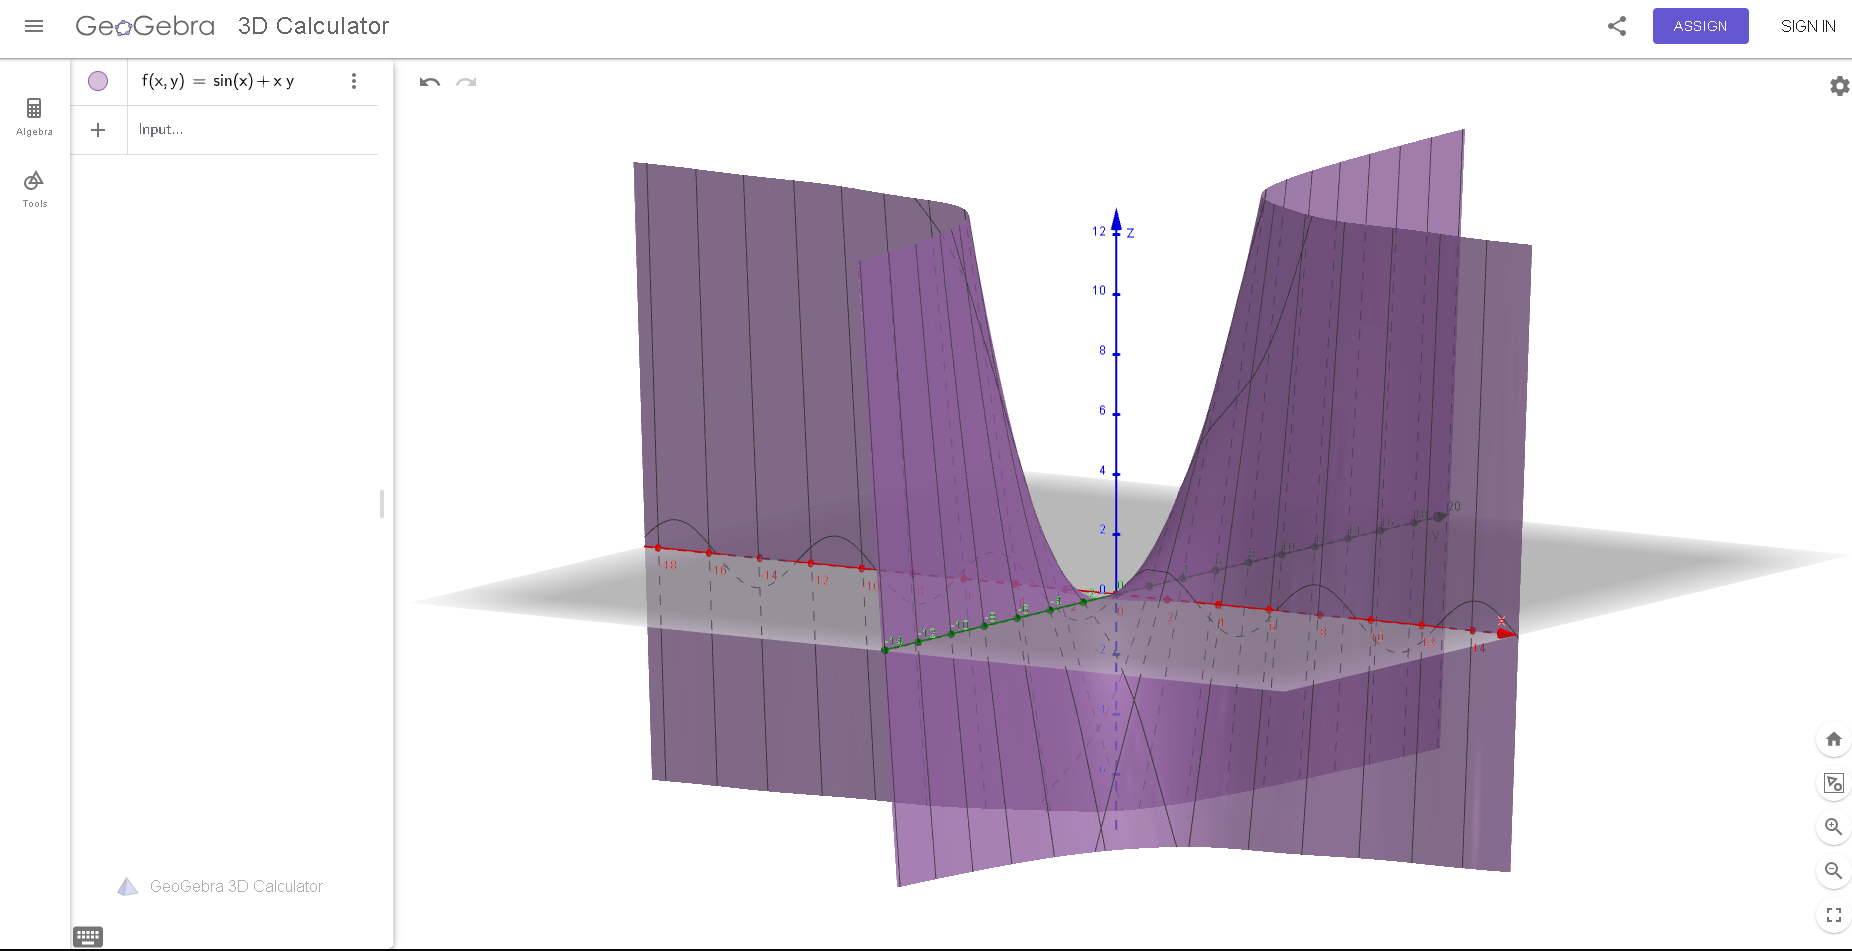
\includegraphics[width=1\linewidth]{Sinx1+x1x2 .png}
    \caption{Model of $f(x_1,x_2) = sinx_1 + x_1x_2$}
    \label{fig:fx1,x2}
\end{figure}
\vspace{2em}
Consider a single perceptron attempting to approximate the function
$f(x_1, x_2) = \sin(x_1) + x_1 x_2$ at the point $x_1 = 0.6$,
$x_2 = 0.9$. The true value is:

\begin{align*}
    f(0.6,\ 0.9) &= \sin(0.6) + (0.6)(0.9) \\
                 &= 0.565 + 0.540 \\
                 &= 1.105
\end{align*}

\noindent The perceptron has weights $w_1 = -0.8$, $w_2 = 1.5$, and bias
$b = -0.3$. The pre-activation is the same regardless of which activation
function is used:

\begin{align*}
    z &= w_1 x_1 + w_2 x_2 + b \\
      &= (-0.8)(0.6) + (1.5)(0.9) + (-0.3) \\
      &= -0.48 + 1.35 - 0.30 \\
      &= 0.57
\end{align*}

\noindent\textbf{Sigmoid}

\begin{align*}
    a &= \frac{1}{1 + e^{-z}}
       = \frac{1}{1 + e^{-0.57}}
       = \frac{1}{1.566}
       \approx 0.639
\end{align*}

\noindent\textbf{Tanh}

\begin{align*}
    a &= \tanh(z)
       = \frac{e^{0.57} - e^{-0.57}}{e^{0.57} + e^{-0.57}}
       = \frac{1.768 - 0.566}{1.768 + 0.566}
       = \frac{1.202}{2.334}
       \approx 0.515
\end{align*}

\noindent The approximation errors against the true value
$f(0.6,\ 0.9) = 1.105$ are:

\begin{align*}
    \varepsilon_{\text{sigmoid}}
        &= |1.105 - 0.639| = 0.466
        \quad \left( \approx 42\% \text{ relative error} \right) \\
    \varepsilon_{\text{tanh}}
        &= |1.105 - 0.515| = 0.590
        \quad \left( \approx 53\% \text{ relative error} \right)
\end{align*}

 As you can see the error is structural, even if the weights are adjusted it wouldn't yield the desired result. As both of the sigmoid function and tanh function have a range of (0,1) and (-1,1) respectively. 
 

What does this value mean when going back to the original function approximation? Well, for the case of one perceptron its just a perdition point of where the function is at this respective input.

However this is not the final step in a Neural network, the output from a perceptron (in hidden layer) is then passed through an output node.(see section \ref{sec:mlp} for better understanding)

This process is done at each node in the \emph{hidden layer}. The output is then used for the neural network to make a prediction.

One perceptron in not enough for approximating complex functions, thus we add more for our prediction to become more accurate. This gave rise to the \emph{Multi layer perceptron}, where each layer plays its own role. \citep{minsky1969}


\newpage
\section{Multi Layer Perceptrons}
\label{sec:mlp}
% ══════════════════════════════════════════════════════════════════════════════

A \emph{multi layer perceptron} (MLP) is the foundational architecture of modern
neural networks and the building block on which Physics-Informed Neural Networks
are constructed.

In the following section we will refer to a perceptron as a \emph{neuron or node} as the name perceptron historically is attributed to usage of the step function which is not in our current focus but is a useful starting point. 

\subsection{Why are multiple Perceptrons Needed? — The Nonlinearity Problem}
\label{sec:nonlinearity}

For simple linearly separable problems, a single perceptron  is sufficient. Imagine a dataset of points on a graph, if
all points of class A sit on one side and all points of class B on the other, a single straight line separates them perfectly (Figure~\ref{fig:xor_problem}a). The perceptron
learns the equation of that line through its weights $w_i$ and bias $b$.

However, many real-world problems are not linearly separable. Consider a dataset where
class A points cluster in two opposite corners of the graph, and class B points cluster
in the other two, where no single straight line can separate them
(Figure~\ref{fig:xor_problem}b). This is the classical \emph{XOR problem}, used by
Minsky and Papert \citep{minsky1969} to expose the limits of a single-layer perceptron.
\begin{figure}[H]
\centering
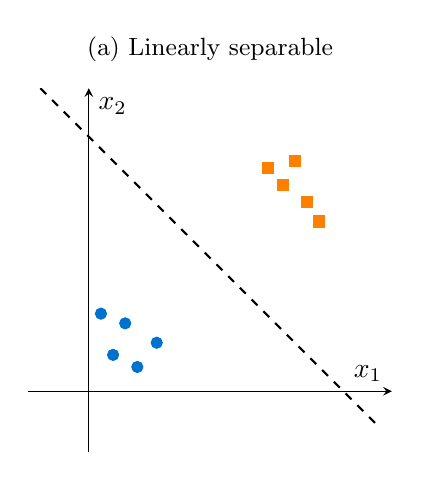
\begin{tikzpicture}
\begin{axis}[
    width=6.2cm, height=6.2cm, axis lines=middle,
    xlabel={$x_1$}, ylabel={$x_2$},
    xmin=-0.25, xmax=1.25, ymin=-0.25, ymax=1.25,
    xtick=\empty, ytick=\empty,
    title={(a) Linearly separable}, title style={font=\small}]
\addplot[only marks, mark=*, mark size=2pt, color=accentblue]
    coordinates {(0.10,0.15)(0.20,0.10)(0.15,0.28)(0.05,0.32)(0.28,0.20)};
\addplot[only marks, mark=square*, mark size=2pt, color=orange]
    coordinates {(0.80,0.85)(0.90,0.78)(0.74,0.92)(0.95,0.70)(0.85,0.95)};
\addplot[domain=-0.2:1.2, thick, dashed, color=black] {1.05 - x};
\end{axis}
\end{tikzpicture}
\hspace{0.6cm}
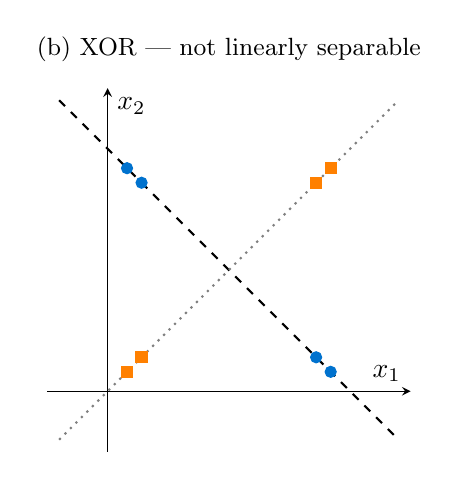
\begin{tikzpicture}
\begin{axis}[
    width=6.2cm, height=6.2cm, axis lines=middle,
    xlabel={$x_1$}, ylabel={$x_2$},
    xmin=-0.25, xmax=1.25, ymin=-0.25, ymax=1.25,
    xtick=\empty, ytick=\empty,
    title={(b) XOR --- not linearly separable}, title style={font=\small}]
\addplot[only marks, mark=*, mark size=2pt, color=accentblue]
    coordinates {(0.08,0.92)(0.92,0.08)(0.14,0.86)(0.86,0.14)};
\addplot[only marks, mark=square*, mark size=2pt, color=orange]
    coordinates {(0.08,0.08)(0.92,0.92)(0.14,0.14)(0.86,0.86)};
\addplot[domain=-0.2:1.2, thick, dashed, color=black] {1.0 - x};
\addplot[domain=-0.2:1.2, thick, dotted, color=gray] {x};
\end{axis}
\end{tikzpicture}
\caption{(a) Linearly separable.  (b) Non-linearly separable.}
\label{fig:xor_problem}
\end{figure}


Since one perceptron can only produce one bend for each activation function, staking multiples of them in parallel in a layer allows us to create more bends to further better our approximation of the function. Each additional layer allows
the network to draw one more \emph{curved} or \emph{composite} decision boundary. With
enough neurons and layers, the network can separate arbitrarily complex data
distributions --- the universal approximation theorem formalises this result
\citep{hornik1989, cybenko1989,leshno1993}. 

Fig.3 is an example of how perceptron produces only a one bend using the tanh (explained in section 2) and how adding just a couple more gives us more bends to better approximate a function. Without these activation functions we would only have a linear line $wx + b$ and no usefull function. 



\begin{figure}[H]
\centering
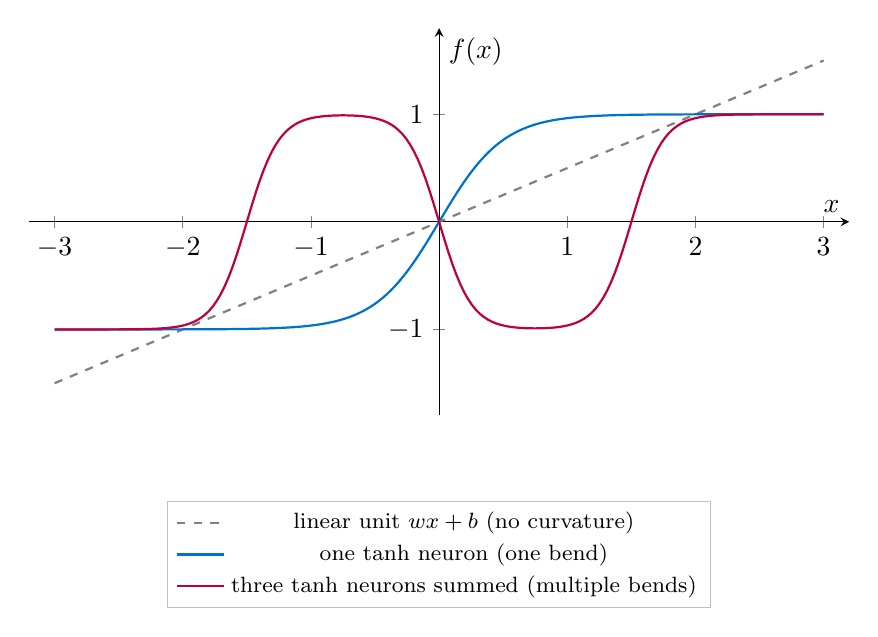
\begin{tikzpicture}
\begin{axis}[
    width=12cm, height=6.5cm, axis lines=middle,
    xlabel={$x$}, ylabel={$f(x)$},
    xmin=-3.2, xmax=3.2, ymin=-1.8, ymax=1.8,
    legend style={at={(0.5,-0.22)}, anchor=north, font=\footnotesize, draw=gray!50},
    legend columns=1, samples=200,
    declare function={mytanh(\x)=2/(1+exp(-2*\x))-1;}]
\addplot[domain=-3:3, thick, dashed, color=gray] {0.5*x};
\addlegendentry{linear unit $wx+b$ (no curvature)}
\addplot[domain=-3:3, thick, color=accentblue] {mytanh(2*x)};
\addlegendentry{one $\tanh$ neuron (one bend)}
\addplot[domain=-3:3, thick, color=purple]
    {mytanh(4*(x+1.5)) - mytanh(4*x) + mytanh(4*(x-1.5))};
\addlegendentry{three $\tanh$ neurons summed (multiple bends)}
\end{axis}
\end{tikzpicture}
\caption{
$\tanh$ neuron contributes one bend; summing several neurons superposes their bends so
the output approximates an increasingly complex curve.}
\label{fig:curvature}
\end{figure}


To better show this lets look at Fig. ~\ref{fig:placeholder}, where we can see how adding more neurons in a neural network allows it to approximate a simple function such as $f(x) = sinx$ much more accurately. 
\begin{figure}[H]
    \centering
    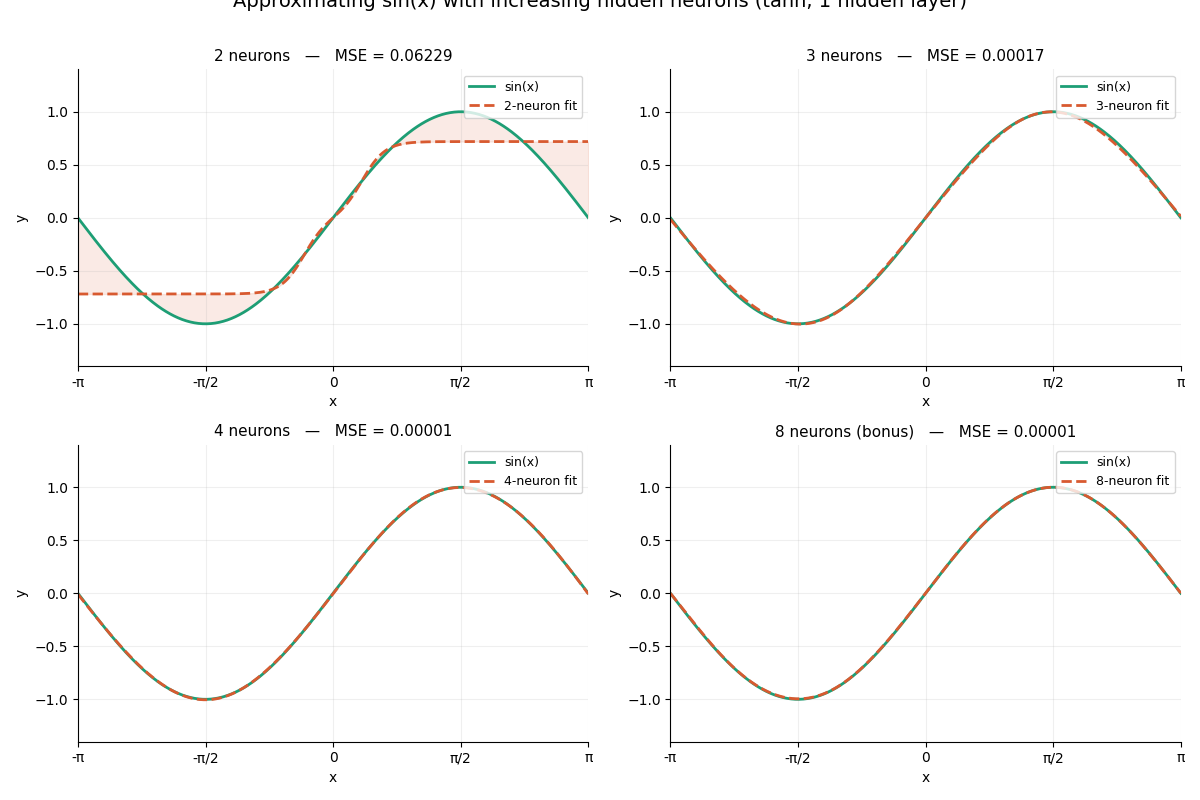
\includegraphics[width=1\linewidth]{Sinx example.png}
    \caption{Approximating the Sinx function by adding multiple neurons }
    \label{fig:placeholder}
\end{figure}


\newpage
\subsection{Architecture}

An MLP consists of an ordered sequence of \emph{layers}, each containing a set of
neurons. Three layer types are distinguished:

\begin{itemize}
    \item \textbf{Input layer}: receives the raw input features.
    \item \textbf{Hidden layers}: one or more intermediate layers that learn internal representations. All neurons in one layer are connected to all neurons in the next.
    \item \textbf{Output layer}: produces the final prediction. 
\end{itemize}

\begin{figure}[H]
\centering
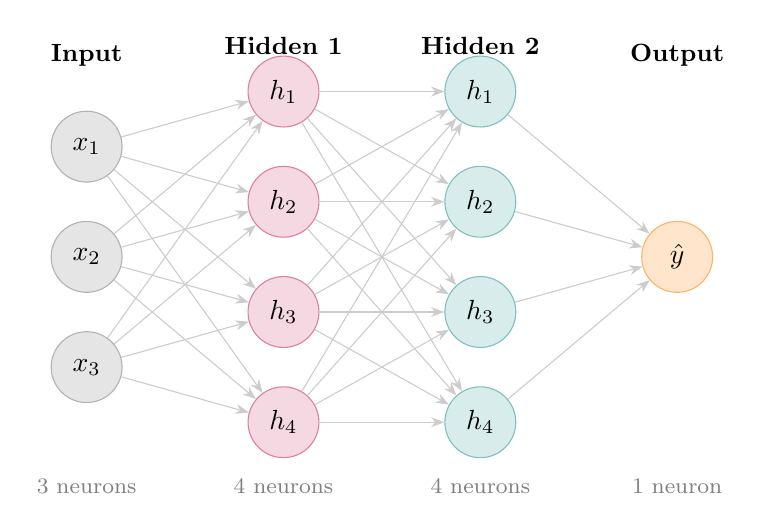
\begin{tikzpicture}[
    node distance = 1.4cm,
    neuron/.style = {circle, draw, minimum size = 0.9cm, inner sep = 0pt},
    input neuron/.style   = {neuron, fill=gray!20,   draw=gray!60},
    hidden neuron/.style  = {neuron, fill=purple!15,  draw=purple!50},
    hidden2 neuron/.style = {neuron, fill=teal!15,    draw=teal!50},
    output neuron/.style  = {neuron, fill=orange!20,  draw=orange!60},
    >=Stealth
]
\foreach \i in {1,2,3}{
    \node[input neuron]  (I-\i)  at (0,   -\i*1.4)        {$x_{\i}$}; }
\foreach \i in {1,2,3,4}{
    \node[hidden neuron] (H1-\i) at (2.5,  -\i*1.4 + 0.7) {$h_{\i}$}; }
\foreach \i in {1,2,3,4}{
    \node[hidden2 neuron](H2-\i) at (5.0,  -\i*1.4 + 0.7) {$h_{\i}$}; }
\node[output neuron] (O-1) at (7.5, -2.8) {$\hat{y}$};

\foreach \i in {1,2,3}{
    \foreach \j in {1,2,3,4}{
        \draw[gray!40, ->] (I-\i) -- (H1-\j); }}
\foreach \i in {1,2,3,4}{
    \foreach \j in {1,2,3,4}{
        \draw[gray!40, ->] (H1-\i) -- (H2-\j); }}
\foreach \i in {1,2,3,4}{
    \draw[gray!40, ->] (H2-\i) -- (O-1); }

\node[above, font=\small\bfseries] at (0,   -0.50) {Input};
\node[above, font=\small\bfseries] at (2.5, -0.35) {Hidden 1};
\node[above, font=\small\bfseries] at (5.0, -0.35) {Hidden 2};
\node[above, font=\small\bfseries] at (7.5, -0.50) {Output};

\node[below, font=\footnotesize, text=gray] at (0,   -5.5) {3 neurons};
\node[below, font=\footnotesize, text=gray] at (2.5, -5.5) {4 neurons};
\node[below, font=\footnotesize, text=gray] at (5.0, -5.5) {4 neurons};
\node[below, font=\footnotesize, text=gray] at (7.5, -5.5) {1 neuron};
\end{tikzpicture}
\caption{Architecture of an MLP with one input layer (3 neurons), two hidden layers
(4 neurons each), and one output layer. Every neuron in a layer connects to every
neuron in the next layer.}
\label{fig:mlp_architecture}
\end{figure}

The \emph{input layer} carries forward the sum of the inputs with their respective weights $w_ix_i$ and the neuron's respective bias $b_j$. 

The \emph{hidden layer} recives the weighted sum value from the previous layer and then passes it through an activation function which introduces the non linearity needed. 

In the \emph{output layer} the output of the hidden layer is then multiplied by sizing factor to get a better approximation of the wanted function. Without this layer we would face issues as the one we had with the example of \ref{sinx + x1x2 example} $f(x_1,x_2) = sinx_1 + x_1x_2$. 



\subsubsection{Multiple neurons and layers} 


The question now is how does having an activation function with multiple neurons together give us a better estimate. Lets take a look at our example from before for the function of $f(x_1,x_2) = sinx_1 +  x_1x_2$. We already saw what the output is for a single neurone, now lets look at a standard Neural network. 

\begin{figure}[H]


% ---- (a) Case 1 ------------------------------------------------
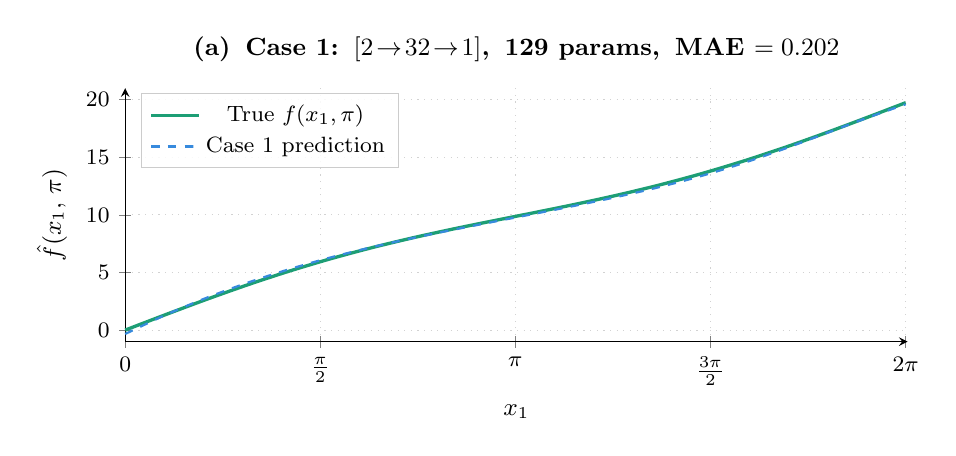
\begin{tikzpicture}
\begin{axis}[
  approxstyle,
  ylabel={$\hat{f}(x_1,\,\pi)$},
  title={(a)\enspace Case~1:\enspace
         $[2\!\to\!32\!\to\!1]$,\enspace
         129 params,\enspace MAE $= 0.202$}
]
\addplot[col-teal, very thick, smooth] coordinates {
  (0.0000,0.0000)(0.3307,1.3636)(0.6614,2.6920)(0.9921,3.9539)
  (1.3228,5.1250)(1.6535,6.1911)(1.9842,7.1492)(2.3149,8.0081)
  (2.6456,8.7872)(2.9762,9.5147)(3.3069,10.2245)(3.6376,10.9520)
  (3.9683,11.7311)(4.2990,12.5900)(4.6297,13.5481)(4.9604,14.6142)
  (5.2911,15.7853)(5.6218,17.0472)(5.9525,18.3756)(6.2832,19.7392)
};
\addlegendentry{True $f(x_1,\pi)$}

\addplot[col-blue, dashed, thick, smooth] coordinates {
  (0.0000,-0.3367)(0.3307,1.3429)(0.6614,2.8312)(0.9921,4.1400)
  (1.3228,5.2919)(1.6535,6.3044)(1.9842,7.1944)(2.3149,7.9885)
  (2.6456,8.7210)(2.9762,9.4237)(3.3069,10.1207)(3.6376,10.8317)
  (3.9683,11.5818)(4.2990,12.4073)(4.6297,13.3496)(4.9604,14.4388)
  (5.2911,15.6724)(5.6218,17.0016)(5.9525,18.3413)(6.2832,19.5998)
};
\addlegendentry{Case~1 prediction}
\end{axis}
\end{tikzpicture}

\vspace{2pt}

% ---- (b) Case 2 ------------------------------------------------
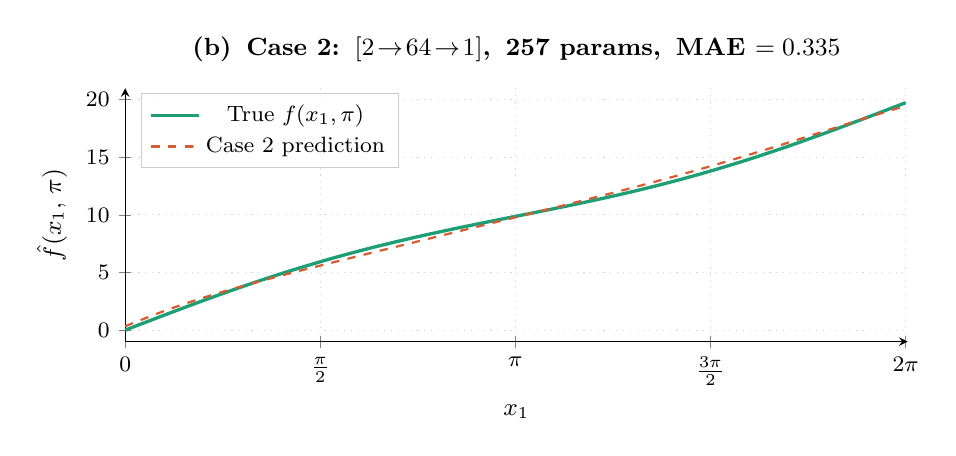
\begin{tikzpicture}
\begin{axis}[
  approxstyle,
  ylabel={$\hat{f}(x_1,\,\pi)$},
  title={(b)\enspace Case~2:\enspace
         $[2\!\to\!64\!\to\!1]$,\enspace
         257 params,\enspace MAE $= 0.335$}
]
\addplot[col-teal, very thick, smooth] coordinates {
  (0.0000,0.0000)(0.3307,1.3636)(0.6614,2.6920)(0.9921,3.9539)
  (1.3228,5.1250)(1.6535,6.1911)(1.9842,7.1492)(2.3149,8.0081)
  (2.6456,8.7872)(2.9762,9.5147)(3.3069,10.2245)(3.6376,10.9520)
  (3.9683,11.7311)(4.2990,12.5900)(4.6297,13.5481)(4.9604,14.6142)
  (5.2911,15.7853)(5.6218,17.0472)(5.9525,18.3756)(6.2832,19.7392)
};
\addlegendentry{True $f(x_1,\pi)$}

\addplot[col-coral, dashed, thick, smooth] coordinates {
  (0.0000,0.3375)(0.3307,1.7249)(0.6614,2.9196)(0.9921,3.9655)
  (1.3228,4.9182)(1.6535,5.8235)(1.9842,6.7099)(2.3149,7.5904)
  (2.6456,8.4690)(2.9762,9.3472)(3.3069,10.2283)(3.6376,11.1194)
  (3.9683,12.0314)(4.2990,12.9775)(4.6297,13.9701)(4.9604,15.0164)
  (5.2911,16.1131)(5.6218,17.2429)(5.9525,18.3749)(6.2832,19.4698)
};
\addlegendentry{Case~2 prediction}
\end{axis}
\end{tikzpicture}

\vspace{2pt}

% ---- (c) Case 3 ------------------------------------------------
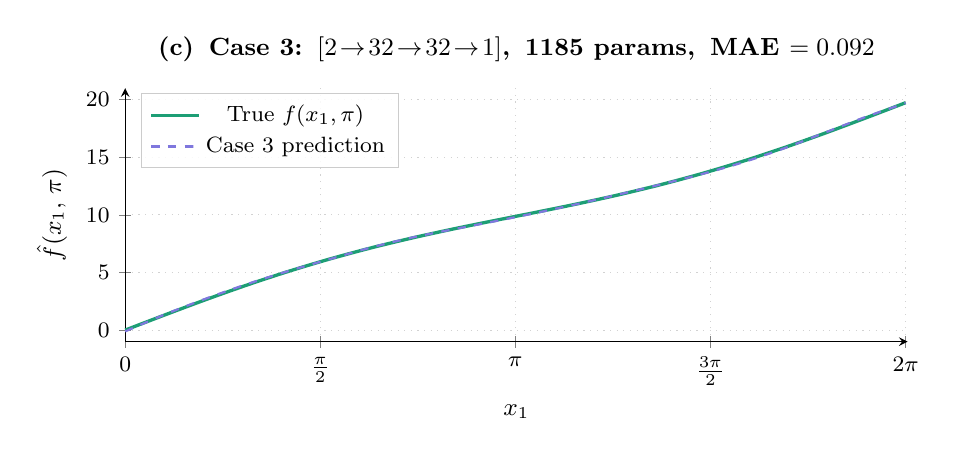
\begin{tikzpicture}
\begin{axis}[
  approxstyle,
  ylabel={$\hat{f}(x_1,\,\pi)$},
  title={(c)\enspace Case~3:\enspace
         $[2\!\to\!32\!\to\!32\!\to\!1]$,\enspace
         1185 params,\enspace MAE $= 0.092$}
]
\addplot[col-teal, very thick, smooth] coordinates {
  (0.0000,0.0000)(0.3307,1.3636)(0.6614,2.6920)(0.9921,3.9539)
  (1.3228,5.1250)(1.6535,6.1911)(1.9842,7.1492)(2.3149,8.0081)
  (2.6456,8.7872)(2.9762,9.5147)(3.3069,10.2245)(3.6376,10.9520)
  (3.9683,11.7311)(4.2990,12.5900)(4.6297,13.5481)(4.9604,14.6142)
  (5.2911,15.7853)(5.6218,17.0472)(5.9525,18.3756)(6.2832,19.7392)
};
\addlegendentry{True $f(x_1,\pi)$}

\addplot[col-purple, dashed, thick, smooth] coordinates {
  (0.0000,-0.1155)(0.3307,1.4095)(0.6614,2.7800)(0.9921,4.0350)
  (1.3228,5.1556)(1.6535,6.1813)(1.9842,7.1856)(2.3149,8.0480)
  (2.6456,8.7573)(2.9762,9.4462)(3.3069,10.1694)(3.6376,10.9383)
  (3.9683,11.7585)(4.2990,12.6116)(4.6297,13.5060)(4.9604,14.5165)
  (5.2911,15.7215)(5.6218,17.0927)(5.9525,18.4713)(6.2832,19.7059)
};
\addlegendentry{Case~3 prediction}
\end{axis}
\end{tikzpicture}

\caption{Approximation of $f(x_1, x_2) = \sin(x_1) + x_1 x_2$}
\label{fig:approx_cases}
\end{figure}

\begin{figure}[H]
\centering
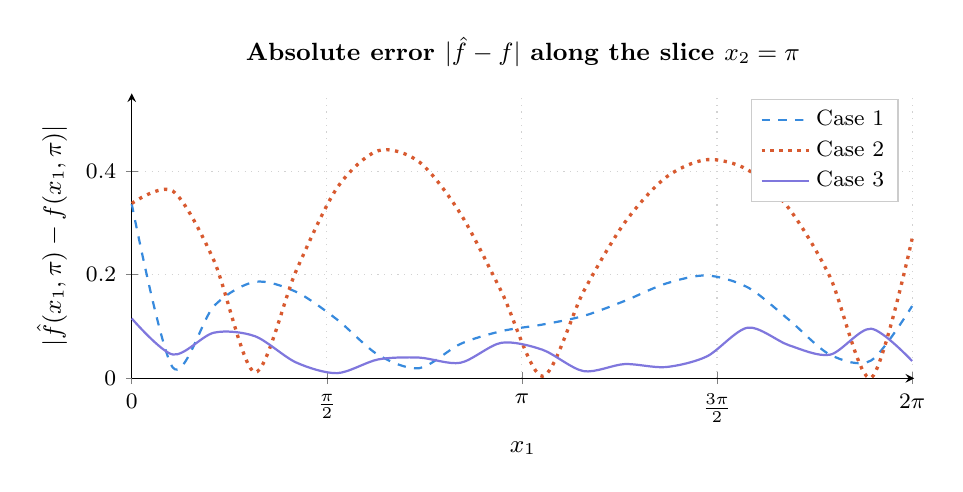
\begin{tikzpicture}
\begin{axis}[
  width=0.95\linewidth,
  height=5.2cm,
  axis lines=left,
  grid=major,
  grid style={dotted,gray!35},
  tick label style={font=\footnotesize},
  label style={font=\small},
  title style={font=\small\bfseries},
  title={Absolute error $|\hat{f} - f|$ along the slice $x_2 = \pi$},
  xlabel={$x_1$},
  ylabel={$|\hat{f}(x_1,\pi) - f(x_1,\pi)|$},
  xmin=0, xmax=6.30,
  ymin=0, ymax=0.55,
  xtick={0,1.5708,3.1416,4.7124,6.2832},
  xticklabels={$0$,$\frac{\pi}{2}$,$\pi$,$\frac{3\pi}{2}$,$2\pi$},
  legend style={
    font=\footnotesize,
    at={(0.98,0.98)},
    anchor=north east,
    draw=gray!40
  },
  clip=false
]

\addplot[col-blue, dashed, thick, smooth] coordinates {
  (0.0000,0.3367)(0.3307,0.0207)(0.6614,0.1392)(0.9921,0.1861)
  (1.3228,0.1669)(1.6535,0.1133)(1.9842,0.0452)(2.3149,0.0195)
  (2.6456,0.0662)(2.9762,0.0910)(3.3069,0.1037)(3.6376,0.1203)
  (3.9683,0.1493)(4.2990,0.1827)(4.6297,0.1985)(4.9604,0.1754)
  (5.2911,0.1130)(5.6218,0.0456)(5.9525,0.0343)(6.2832,0.1394)
};
\addlegendentry {Case 1}

\addplot[col-coral, dotted, very thick, smooth] coordinates {
  (0.0000,0.3375)(0.3307,0.3613)(0.6614,0.2275)(0.9921,0.0116)
  (1.3228,0.2069)(1.6535,0.3676)(1.9842,0.4393)(2.3149,0.4176)
  (2.6456,0.3182)(2.9762,0.1675)(3.3069,0.0039)(3.6376,0.1674)
  (3.9683,0.3002)(4.2990,0.3875)(4.6297,0.4220)(4.9604,0.4023)
  (5.2911,0.3278)(5.6218,0.1958)(5.9525,0.0007)(6.2832,0.2694)
};
\addlegendentry{Case~2 }

\addplot[col-purple, thick, smooth] coordinates {
  (0.0000,0.1155)(0.3307,0.0459)(0.6614,0.0880)(0.9921,0.0812)
  (1.3228,0.0306)(1.6535,0.0099)(1.9842,0.0364)(2.3149,0.0399)
  (2.6456,0.0299)(2.9762,0.0685)(3.3069,0.0551)(3.6376,0.0138)
  (3.9683,0.0274)(4.2990,0.0216)(4.6297,0.0421)(4.9604,0.0977)
  (5.2911,0.0638)(5.6218,0.0455)(5.9525,0.0957)(6.2832,0.0333)
};
\addlegendentry{Case~3 }

\end{axis}
\end{tikzpicture}
\caption{Absolute error for each case}
\label{fig:error_curves}
\end{figure}


\paragraph{Observation} Case~2 shows the largest and most
oscillatory errors. Case~3 consistently achieves the
smallest error, showing that adding more layers is more effective than just adding more neurons in a single layer in in this case.

If adding more layers makes the network prediction much more accurate, why not just keep adding layers until we get a highly accurate morel?

\begin{itemize}
    \item Vanishing gradient problem \citep{bengio1994}
    \item Computational costs
    \item Overfitting\citep{srivastava2014}
\end{itemize}

After a certain number of layers, it becomes pointless and/or damaging to add in more layers. When designing a neural the "depth" of the network must be specific to the task at hand.

\section{Data types}

Now that we understand the structure of a NN, lets see what they can be used for. 

Input data is usually numbers, but numbers can be representative of many things. For example the number "2" can represent 2 hours, minutes, kilometers or a coordinate. The NN does not see units but only takes in integers, this means as long as we can represent the data as an integer the neural network can accept it. 

\subsection{Images}
\subsection{Simple data types}
\subsection{Combining data types and why non-dimentionalization matters}
\section{types of neural network and their summuries}


\subsection{Fourier Feature Embeddings}
\label{sec:ffe}

\subsubsection{Why Does a Standard MLP Struggle with Sharp Gradients?}

Standard MLPs exhibit \emph{spectral bias}: gradient descent preferentially fits
low-frequency components first and converges slowly on high-frequency spatial
variations \citep{tancik2020}. For the NiTi wire problem, the sharp thermal
gradient near the wire ends — decaying over characteristic length
$L_b \approx \sqrt{kR/2h} \approx 9.5\,\text{mm}$ — must be captured faithfully.
A plain MLP fits the bulk temperature field accurately but smears this end gradient.

\subsubsection{What Are Fourier Feature Embeddings?}

The remedy is to transform the raw input coordinates before feeding them to the
network \citep{tancik2020}:

\begin{equation}
    \boldsymbol{\gamma}(\mathbf{x}^*)
    =
    \begin{bmatrix}
        \sin(2\pi\,\mathbf{B}_1 \cdot \mathbf{x}^*)\\
        \cos(2\pi\,\mathbf{B}_1 \cdot \mathbf{x}^*)\\
        \vdots\\
        \sin(2\pi\,\mathbf{B}_m \cdot \mathbf{x}^*)\\
        \cos(2\pi\,\mathbf{B}_m \cdot \mathbf{x}^*)
    \end{bmatrix}
    \label{eq:ffe}
\end{equation}

where $\mathbf{x}^* = (x^*, r^*, t^*)$ are the nondimensionalised input
coordinates and $\mathbf{B} \in \mathbb{R}^{m \times 3}$ is a fixed random
frequency matrix sampled once from $\mathcal{N}(0, \sigma^2)$ before training
and held frozen throughout.

$\mathbf{B}$ fixes the frequencies available to the network — analogous to
integer harmonics in a classical Fourier series. The MLP weights that follow
$\boldsymbol{\gamma}$ learn the amplitudes of those basis functions, playing the
role of Fourier coefficients. Because the high-frequency basis functions are
explicitly present in the input before training begins, the network is no longer
required to generate high-frequency variation from smooth activations. The standard
deviation $\sigma \approx 1$--$10$ in nondimensional coordinates is typical for
thermal field problems.


\section{The loss function and how the neural network updates its prediction}

Lets look again at our example \ref{sinx + x1x2 example} and fig \ref{fig:approx_cases}. in the figure you can see the number of parameters run or what is normally called \textit{epoch}. This represents the number of cycles that the NN went through to finally arrive at a statisfying or equal vale, where $|y - y*| = 0 $ or at least very close to 0. 

But how does this cycle updates? when we get an error from out first prediction, we understand that this value came to be due to a wrong distribution of weights from the input layer. We use the error value to adjust our weights $w$. Think about adjusting a knob for each weight for a signal until you get the shape that you want. 

To understand loss functions and their types, we need to know what \textit{backpropagation}. A process that is used to update the value of the weight with each iteration in relation to the error that we get at said iteration.
% ══════════════════════════════════════════════════════════════════════════════
\subsection{Backpropagation and Automatic Differentiation}
\label{sec:autodiff}
% ══════════════════════════════════════════════════════════════════════════════

Two distinct differentiation processes operate inside a Neural Network. The first is
\emph{backpropagation}, which computes how the loss changes with respect to the
network weights $\theta$. The second is \emph{automatic differentiation} (autodiff),
which computes how the network output changes with respect to its coordinate inputs
$(x^*, r^*, t^*)$. Both use the chain rule of calculus but ask different questions.\citep{rumelhart1986}
% ============================================================
%  Automatic Differentiation
%  Section for the PINNs Tutorial
% ============================================================



Automatic differentiation (AD) is a technique that is central to machine
learning, neural networks, and many other computational fields.
AD yields the \emph{exact} derivative of a function  to floating-point
precision regardless of how complex that function is, and it does so at a
computational cost proportional to a single forward evaluation of the
function.

The two classical alternatives both have significant limitations when
executed on a computer.
\emph{Finite differences} accumulate round-off error -- the error grows as the
step size $h$ is reduced and require multiple function evaluations per
derivative.
\emph{Symbolic differentiation} is exact in principle but suffers from
\emph{expression swell}: the size of the symbolic expression grows
exponentially with the number of operations, making it impractical for deep networks.
~\citep{baydin2018} gave a systematic comparison of all
three methods; Table~1 in Section~3.3.3 of this document reproduces the key
numerical results.

AD avoids both problems by applying the chain rule to each elementary
operation in the computation graph, accumulating exact numerical derivative
values rather than symbolic expressions.

% ---------------------------------------------------------------
\subsubsection{The Chain Rule and Intermediate Variables}
% ---------------------------------------------------------------

AD uses the chain rule applied to composite functions.
Consider a scalar function built by composing three operations:

\begin{equation}
  y = f\!\bigl(g\!\bigl(h(x)\bigr)\bigr).
\end{equation}

Introduce intermediate variables $\omega_0, \omega_1, \omega_2, \omega_3$
that name each intermediate quantity:

\begin{equation}
  \omega_0 = x, \qquad
  \omega_1 = h(\omega_0), \qquad
  \omega_2 = g(\omega_1), \qquad
  \omega_3 = f(\omega_2) = y.
\end{equation}

The chain rule then gives the total derivative of $y$ with respect to $x$
as a product of local partial derivatives:

\begin{equation}
  \frac{\mathrm{d}y}{\mathrm{d}x}
  = \frac{\partial f(\omega_2)}{\partial \omega_2}
    \cdot \frac{\partial g(\omega_1)}{\partial \omega_1}
    \cdot \frac{\partial h(\omega_0)}{\partial \omega_0}.
  \label{eq:ad_chain}
\end{equation}

At each node in the computation graph, only the \emph{local} partial
derivative -- the derivative of that node's output with respect to its own
input -- is needed.
This local quantity is computed exactly and stored numerically; the full
derivative is the accumulated product of all such local values along the
path from input to output.

% ---------------------------------------------------------------
% ---------------------------------------------------------------

Equation~\eqref{eq:ad_chain} can be evaluated in two directions, giving rise
to two distinct AD modes.

\subsubsection{Forward Accumulation (FA).}
The product in~\eqref{eq:ad_chain} is evaluated \emph{left to right},
starting from the input $x$ and propagating toward the output $y$.
Define the \emph{tangent} (or \emph{dot}) value of each intermediate variable
as its derivative with respect to the chosen input:

\begin{equation}
  \dot{\omega}_i = \frac{\partial \omega_i}{\partial x}.
\end{equation}

The forward sweep propagates tangents according to:

\begin{equation}
  \frac{\partial \omega_i}{\partial x}
  = \frac{\partial \omega_i}{\partial \omega_{i-1}}
    \cdot \frac{\partial \omega_{i-1}}{\partial x}.
  \label{eq:FA}
\end{equation}

The computation begins with a \emph{seed value} $\dot{\omega}_0 = \partial x / \partial x = 1$
and propagates forward through the graph.
One forward pass yields the derivative of $y$ with respect to \emph{one}
input variable.
For a function of $n$ inputs, $n$ forward passes are required to obtain the
full gradient.

\subsubsection{Backward (Reverse) Accumulation (BA).}
The product is evaluated \emph{right to left}, starting from the output $y$
and propagating toward the inputs.
Define the \emph{adjoint} (or \emph{bar}) value of each intermediate variable
as the derivative of the output with respect to that variable:

\begin{equation}
  \bar{\omega}_i = \frac{\partial y}{\partial \omega_i}.
\end{equation}

The reverse sweep propagates adjoints according to:

\begin{equation}
  \frac{\partial y}{\partial \omega_i}
  = \frac{\partial y}{\partial \omega_{i+1}}
    \cdot \frac{\partial \omega_{i+1}}{\partial \omega_i}.
  \label{eq:BA}
\end{equation}

The computation begins with the seed value $\bar{\omega}_3 = \partial y / \partial y = 1$
and propagates backward through the graph.
One reverse pass yields the derivative of $y$ with respect to \emph{all}
input variables simultaneously.


\subsubsection{Key efficiency result.}
For a scalar output (such as a neural network loss $\mathcal{L}$) and a
large number of inputs (such as millions of network weights $\theta$),
reverse accumulation computes the full gradient $\nabla_\theta \mathcal{L}$
in a single backward pass , but it can only do this at a cost proportional to one forward
evaluation. This means we still have to evaluate the the gradient of each node in the forward pass first.
This is precisely why backpropagation is the algorithm that
makes deep learning computationally feasible.


The tradeoff is memory: the forward pass values at every node must be stored
so that they are available during the backward sweep.
For large computation graphs this can require significant memory.
Mitigation strategies (gradient checkpointing, reversible architectures) are
discussed in the document.

% ---------------------------------------------------------------
\subsection{Worked Example: Forward Accumulation for
             \texorpdfstring{$f(x_1, x_2) = x_1 x_2 + \sin x_1$}{f(x1, x2) = x1 x2 + sin x1}}
% ---------------------------------------------------------------


Consider the function

\begin{equation}
  y = f(x_1, x_2) = x_1 x_2 + \sin x_1.
\end{equation}

Introduce intermediate variables:

\begin{align}
  \omega_1 &= x_1, \notag\\
  \omega_2 &= x_2, \notag\\
  \omega_3 &= \omega_1 \omega_2, \notag\\
  \omega_4 &= \sin \omega_1, \notag\\
  \omega_5 &= \omega_3 + \omega_4 = y. \notag
\end{align}

\subsubsection*{Forward pass: computing $\partial y / \partial x_1$}

To differentiate with respect to $x_1$, initialise the seed values:

\begin{equation}
  \dot{\omega}_1 = \frac{\partial \omega_1}{\partial x_1} = 1, \qquad
  \dot{\omega}_2 = \frac{\partial \omega_2}{\partial x_1} = 0.
\end{equation}

(Setting $\dot{\omega}_2 = 0$ selects $x_1$ as the independent variable;
$x_2$ is treated as a constant for this pass.)
Propagate forward:

\begin{align}
  \dot{\omega}_3
    &= \dot{\omega}_1 \,\omega_2 + \omega_1 \,\dot{\omega}_2
     = 1 \cdot \omega_2 + \omega_1 \cdot 0
     = \omega_2, \\[4pt]
  \dot{\omega}_4
    &= \cos \omega_1 \cdot \dot{\omega}_1
     = \cos \omega_1, \\[4pt]
  \dot{\omega}_5
    &= \dot{\omega}_3 + \dot{\omega}_4
     = \omega_2 + \cos \omega_1.
\end{align}

Therefore:

\begin{equation}
  \frac{\partial y}{\partial x_1} = \omega_2 + \cos \omega_1
  = x_2 + \cos x_1.
\end{equation}

This is the exact result from calculus, obtained by a single forward sweep
through the graph with no symbolic manipulation.

\subsubsection*{Comparison with the computation graph figure}

Figure~\ref{fig:ad_graph} shows the computation graph for this example.
In forward accumulation, tangent values flow \emph{upward} (from inputs to
output); in reverse accumulation, adjoint values flow \emph{downward} (from
output to inputs).

\begin{figure}[h]
\centering
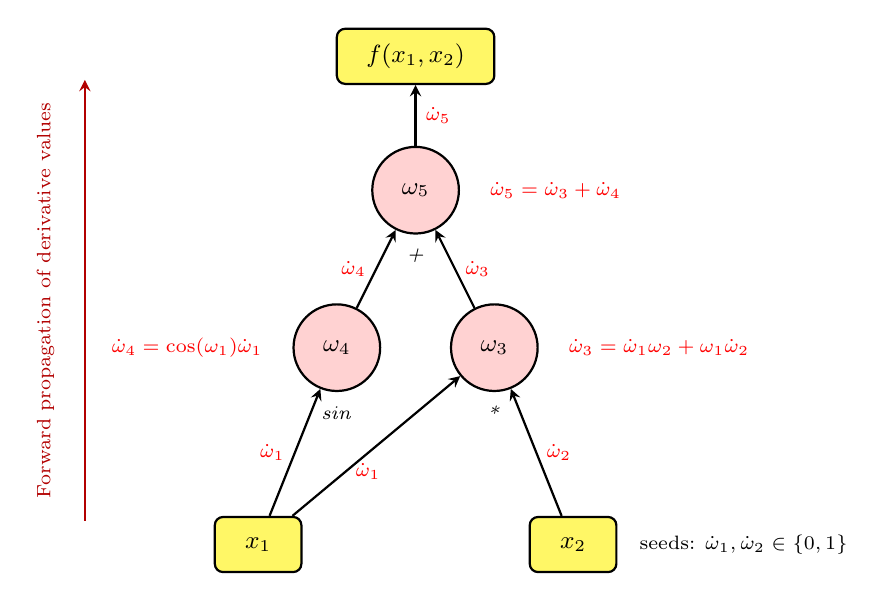
\begin{tikzpicture}[
  inputnode/.style  = {draw, fill=yellow!60, rectangle, rounded corners=3pt,
                        minimum width=1.1cm, minimum height=0.7cm, font=\small},
  opnode/.style     = {draw, fill=pink!70, circle,
                        minimum size=1.1cm, font=\small},
  outputnode/.style = {draw, fill=yellow!60, rectangle, rounded corners=3pt,
                        minimum width=2.0cm, minimum height=0.7cm, font=\small},
  ->, >=stealth, thick
]

% ── Input nodes ──────────────────────────────────────────────────────────────
\node[inputnode] (x1) at (0, 0)   {$x_1$};
\node[inputnode] (x2) at (4, 0)   {$x_2$};

% ── Operation nodes: labelled with wi (primal value) ─────────────────────────
\node[opnode] (sin) at (1, 2.5)   {$\omega_4$};
\node[opnode] (mul) at (3, 2.5)   {$\omega_3$};
\node[opnode] (add) at (2, 4.5)   {$\omega_5$};

% ── Operation type labels (small, below node label) ──────────────────────────
\node[font=\scriptsize, below=0.05cm of sin] {\textit{sin}};
\node[font=\scriptsize, below=0.05cm of mul] {\textit{*}};
\node[font=\scriptsize, below=0.05cm of add] {\textit{+}};

% ── Output node ──────────────────────────────────────────────────────────────
\node[outputnode] (out) at (2, 6.2) {$f(x_1, x_2)$};

% ── Edges: inputs → ops, labelled with tangent values ────────────────────────
\draw (x1) -- node[left,  font=\scriptsize, red] {$\dot\omega_1$} (sin);
\draw (x1) -- node[below, font=\scriptsize, red, pos=0.45] {$\dot\omega_1$} (mul);
\draw (x2) -- node[right, font=\scriptsize, red] {$\dot\omega_2$} (mul);

% ── Edges: ops → add, labelled with tangent values ───────────────────────────
\draw (sin) -- node[left,  font=\scriptsize, red] {$\dot\omega_4$} (add);
\draw (mul) -- node[right, font=\scriptsize, red] {$\dot\omega_3$} (add);

% ── Edge: add → output ───────────────────────────────────────────────────────
\draw (add) -- node[right, font=\scriptsize, red] {$\dot\omega_5$} (out);

% ── Tangent equations beside each operation node ─────────────────────────────
\node[red, font=\scriptsize, right=0.25cm of mul, align=left]
  {$\dot\omega_3 = \dot\omega_1\omega_2 + \omega_1\dot\omega_2$};

\node[red, font=\scriptsize, left=0.25cm of sin, align=right]
  {$\dot\omega_4 = \cos(\omega_1)\dot\omega_1$};

\node[red, font=\scriptsize, right=0.25cm of add, align=left]
  {$\dot\omega_5 = \dot\omega_3 + \dot\omega_4$};

% ── Seed note ────────────────────────────────────────────────────────────────
\node[font=\scriptsize, right=0.15cm of x2, align=left]
  {seeds: $\dot\omega_1, \dot\omega_2 \in \{0,1\}$};

% ── Left-side arrow (adjust x-coord and y-range independently) ───────────────
\draw[->, thick, red!70!black]
  (-2.2, 0.3) -- (-2.2, 5.9);

% ── Left-side label (adjust at independently from the arrow) ─────────────────
\node[font=\scriptsize, red!70!black, rotate=90]
  at (-2.7, 3.1)
  {Forward propagation of derivative values};

\end{tikzpicture}
\caption{Computation graph for forward accumulation applied to
  $f(x_1, x_2) = x_1 x_2 + \sin x_1$.
  Pink circles are operation nodes labelled with their primal value $\omega_i$;
  yellow boxes are inputs and output.
  Red edge labels carry the tangent (dot) values $\dot\omega_i$ propagated
  upward from the seed values $\dot\omega_1, \dot\omega_2 \in \{0,1\}$.}
\label{fig:ad_graph}
\end{figure}
% ---------------------------------------------------------------
\subsection{In Each Step: Numerical Storage}
% ---------------------------------------------------------------

At each node in the graph, the value of the derivative is stored
\emph{numerically} and passed on to the next node.
No symbolic expression is constructed.
This is the property that keeps the computational cost constant regardless
of how many operations compose the function in contrast to symbolic
differentiation, where the expression size grows with each application of the
product or chain rule.

\subsection{The Computation Graph}
\label{sec:compgraph}

Every arithmetic operation a neural network performs is recorded as a node in a
\emph{computation graph}. During the \textbf{forward pass}, values flow left to
right and are stored at each node. During the \textbf{backward pass}, gradients
flow right to left: each node multiplies the incoming gradient by its local
derivative, accumulating the chain-rule product.



\subsection{Worked Example: Two Weights, One Step}

Inputs $x_1 = 1$, $x_2 = 2$; weights $w_1 = w_2 = 0.5$; bias $b = 0$; target
$y = 4$:

\textbf{Forward pass:}
\begin{align}
    z &= 0.5 \times 1 + 0.5 \times 2 = 1.5, \qquad
    \mathcal{L} = (1.5 - 4)^2 = 6.25
\end{align}

\textbf{Backward pass:}
\begin{align}
    \frac{\partial \mathcal{L}}{\partial z} &= 2(1.5-4) = -5.0 \\
    \frac{\partial \mathcal{L}}{\partial w_1} &= -5.0 \times 1 = -5.0, \qquad
    \frac{\partial \mathcal{L}}{\partial w_2}  = -5.0 \times 2 = -10.0
\end{align}

\textbf{Weight update} ($\eta = 0.1$):
\begin{align}
    w_1 \leftarrow 1.0, \qquad w_2 \leftarrow 1.5
\end{align}

\textbf{Verification:} $z' = 1.0 \times 1 + 1.5 \times 2 = 4.0$,
$\mathcal{L}' = 0\;\checkmark$

$w_2$ received a gradient twice as large as $w_1$ because its input $x_2 = 2$
was twice as large as $x_1 = 1$ .\textbf{ Input magnitude directly scales the gradient} a weight receives.

\subsubsection{Worked Example: Two Weights, One Step}

Consider a two-weight network with inputs $x_1 = 1$, $x_2 = 2$, weights
$w_1 = w_2 = 0.5$, bias $b = 0$, and target $y = 4$:

\textbf{Forward pass:}
\begin{align}
    z &= w_1 x_1 + w_2 x_2 + b = 0.5 \times 1 + 0.5 \times 2 + 0 = 1.5
    \label{eq:fwd_z}\\
    \mathcal{L} &= (z - y)^2 = (1.5 - 4)^2 = 6.25
    \label{eq:fwd_L}
\end{align}

\textbf{Backward pass} (applying Eq.~\ref{eq:backprop_chain}):
\begin{align}
    \frac{\partial \mathcal{L}}{\partial z}
    &= 2(z - y) = 2(1.5 - 4) = -5.0
    \label{eq:bwd_dLdz}\\[4pt]
    \frac{\partial \mathcal{L}}{\partial w_1}
    &= \frac{\partial \mathcal{L}}{\partial z}
       \cdot \frac{\partial z}{\partial w_1}
     = -5.0 \times x_1 = -5.0 \times 1 = -5.0
    \label{eq:bwd_w1}\\[4pt]
    \frac{\partial \mathcal{L}}{\partial w_2}
    &= \frac{\partial \mathcal{L}}{\partial z}
       \cdot \frac{\partial z}{\partial w_2}
     = -5.0 \times x_2 = -5.0 \times 2 = -10.0
    \label{eq:bwd_w2}
\end{align}

\textbf{Weight update} with learning rate $\eta = 0.1$:
\begin{align}
    w_1 &\leftarrow 0.5 - 0.1 \times (-5.0) = 1.0
    \label{eq:update_w1}\\
    w_2 &\leftarrow 0.5 - 0.1 \times (-10.0) = 1.5
    \label{eq:update_w2}
\end{align}

\textbf{Verification} --- new forward pass after one update:
\begin{equation}
    z' = 1.0 \times 1 + 1.5 \times 2 = 4.0,
    \qquad
    \mathcal{L}' = (4.0 - 4)^2 = 0 \quad \checkmark
    \label{eq:verify}
\end{equation}

Two observations from this example are important for understanding training
behaviour. First, $w_2$ received a gradient twice as large as $w_1$ because its
input $x_2 = 2$ was twice as large as $x_1 = 1$. Neurons connected to larger
inputs receive larger gradient signals and therefore learn faster --- the input
magnitude directly sets the learning speed for each connection. Second, both
gradients are negative because the network predicted too low ($z = 1.5 < y = 4$),
so both weights must increase. The sign of the gradient always points in the
direction that increases the loss; gradient \emph{descent} moves opposite to
this direction.

% ══════════════════════════════════════════════════════════════════════════════

\subsubsection{Example 2 — Sigmoid Neuron}
\label{ex:cs231n_sigmoid}
% ──────────────────────────────────────────────────────────────────────────────

\textit{Source: Karpathy (2016), CS231n Lecture Notes \cite{karpathy2016cs231n}.
Weights $\mathbf{w} = [2, -3, -3]$, inputs $\mathbf{x} = [-1, -2]$.}

\medskip
A sigmoid neuron computes:
\begin{equation}
    f(\mathbf{w}, \mathbf{x})
    = \sigma\!\left(w_0 x_0 + w_1 x_1 + w_2\right)
    = \frac{1}{1 + e^{-(w_0 x_0 + w_1 x_1 + w_2)}}
    \label{eq:sigmoid_neuron}
\end{equation}

\textbf{Forward pass:}
\begin{align}
    \text{dot} &= w_0 x_0 + w_1 x_1 + w_2
               = (2)(-1) + (-3)(-2) + (-3) = 1 \label{eq:sig_dot}\\
    e^{-\text{dot}} &= e^{-1} \approx 0.3679 \label{eq:sig_exp}\\
    1 + e^{-\text{dot}} &\approx 1.3679 \label{eq:sig_add}\\
    \sigma &= \frac{1}{1.3679} \approx \mathbf{0.731} \label{eq:sig_out}
\end{align}

Rather than backpropagating through each of the four primitive gates (negate,
exponentiate, add one, reciprocal), the sigmoid function has a well-known compact
derivative:

\begin{equation}
    \frac{\mathrm{d}\sigma}{\mathrm{d}z} = \sigma(z)\bigl(1 - \sigma(z)\bigr)
    \label{eq:sigmoid_deriv}
\end{equation}

\textbf{Backward pass} (using the grouped sigmoid gradient):
\begin{align}
    \frac{\partial \mathcal{L}}{\partial \,\text{dot}}
    &= \sigma(1 - \sigma) = 0.731 \times 0.269 \approx \mathbf{0.197}
    \label{eq:sig_bwd_dot}\\[4pt]
    \frac{\partial \mathcal{L}}{\partial w_0}
    &= 0.197 \times x_0 = 0.197 \times (-1) = \mathbf{-0.197}
    \label{eq:sig_bwd_w0}\\[4pt]
    \frac{\partial \mathcal{L}}{\partial w_1}
    &= 0.197 \times x_1 = 0.197 \times (-2) = \mathbf{-0.394}
    \label{eq:sig_bwd_w1}\\[4pt]
    \frac{\partial \mathcal{L}}{\partial w_2}
    &= 0.197 \times 1 \phantom{= 0.197 \times (-)} = \mathbf{+0.197}
    \label{eq:sig_bwd_w2}
\end{align}

Note that $w_1$ receives exactly twice the gradient magnitude of $w_0$ because
its input $x_1 = -2$ has twice the magnitude of $x_0 = -1$. This confirms the
general principle established in the simpler example: input magnitude directly
scales the gradient signal that a weight receives.

The compact grouped derivative eq.~\eqref{eq:sigmoid_deriv} is an instance of a
broader strategy: any sub-expression whose derivative has a simpler closed form
than the chain of its primitive gates can be treated as a single gate. Modern
frameworks implement this for all standard activation functions.

% ──────────────────────────────────────────────────────────────────────────────
\subsubsection{Example 3 — Autodiff Exactness:
               \texorpdfstring{$f(x) = \sin(x)\,e^x$}{f(x)=sin(x)*exp(x)}}
\label{ex:autodiff_exact}
% ──────────────────────────────────────────────────────────────────────────────

\text The exact derivative of $\sin(x)e^x$ is a standard product-rule exercise.
The numerical comparison of autodiff against finite differences is adapted from
Baydin et al.\ \cite{baydin2018autodiff}, the survey reference for automatic
differentiation in machine learning.

\medskip
Consider $f(x) = \sin(x)\,e^x$ evaluated at $x = 1$. Three methods are compared.

\textbf{Exact derivative} (product rule):
\begin{equation}
    f'(x) = \cos(x)\,e^x + \sin(x)\,e^x = e^x\bigl(\sin x + \cos x\bigr)
    \label{eq:sinexp_exact}
\end{equation}
\begin{equation}
    f'(1) = e^1\bigl(\sin 1 + \cos 1\bigr)
           = 2.71828\times(0.84147 + 0.54030)
           = \mathbf{3.75623\ldots}
    \label{eq:sinexp_exact_val}
\end{equation}

\textbf{Method 1 — Finite differences} with $h = 10^{-4}$:
\begin{equation}
    \hat{f}'(1) \approx
    \frac{f(1 + 10^{-4}) - f(1)}{10^{-4}}
    = \frac{3.75627\ldots - 3.75559\ldots}{10^{-4}}
    \approx \mathbf{3.75619\ldots}
    \label{eq:sinexp_fd}
\end{equation}
\begin{equation}
    \text{Error} = |3.75623 - 3.75619| \approx 4.5 \times 10^{-5}
    \label{eq:sinexp_fd_err}
\end{equation}

\textbf{Method 2 — Autodiff} (computation graph):

The function decomposes into two primitive nodes:
$u = \sin(x)$ with $\partial u/\partial x = \cos(x)$, and
$v = e^x$ with $\partial v/\partial x = e^x$.
Their product $f = uv$ has derivative:
\begin{equation}
    \frac{\partial f}{\partial x}
    = v \cdot \frac{\partial u}{\partial x} + u \cdot \frac{\partial v}{\partial x}
    = e^x \cos x + \sin x \cdot e^x
    = e^x(\sin x + \cos x)
    = \mathbf{3.75623\ldots}
    \label{eq:sinexp_ad}
\end{equation}
Error $= 0$ (to floating-point precision).

\begin{table}[H]
\centering
\caption{Comparison of differentiation methods for $f'(1)$ where
         $f(x)=\sin(x)\,e^x$. Exact value: $3.756234\ldots$}
\label{tab:diff_comparison}
\begin{tabularx}{\textwidth}{lXXX}
\toprule
\textbf{Method} & \textbf{Result} & \textbf{Error} & \textbf{Cost for $\partial^2 f/\partial x^2$} \\
\midrule
Finite differences ($h=10^{-4}$)
    & $3.75619\ldots$
    & $\sim 4.5 \times 10^{-5}$
    & 4 network evaluations, error $\mathcal{O}(h)$ \\
Symbolic differentiation
    & $3.75623\ldots$
    & $0$
    & Expression size grows exponentially \\
Automatic differentiation
    & $3.75623\ldots$
    & $0$
    & 1 graph traversal, $\mathcal{O}(\text{forward pass})$ \\
\bottomrule
\end{tabularx}
\end{table}

For the PINN in this thesis, the PDE residual requires $\partial^2 T^*/\partial
x^{*2}$ evaluated at every collocation point. At $N_c = 10{,}000$ collocation
points, finite differences would require $4 N_c = 40{,}000$ network forward passes
per training iteration, each introducing $\mathcal{O}(h)$ truncation error that
accumulates across the PDE loss. Autodiff computes all $N_c$ second derivatives in
a single backward graph traversal at machine precision. This is not a minor
optimisation: it is the difference between a computationally feasible and an
infeasible training procedure.






% ══════════════════════════════════════════════════════════════════════════════
\
% ══════════════════════════════════════════════════════════════════════════════
\section{Nondimensionalisation}
\label{sec:nondim}
% ══════════════════════════════════════════════════════════════════════════════

Before training, every coordinate and physical quantity must be rescaled so that
all network inputs and outputs are $\mathcal{O}(1)$.

\subsection{Why Nondimensionalisation Matters}
\label{sec:nondim_why}

The raw dimensional inputs to the NiTi wire PINN differ by up to four orders of
magnitude ($x \sim 10^{-2}$~m, $r \sim 10^{-4}$~m, $t \sim 10$~s,
$T \sim 300$--$400$~K), causing two distinct problems.

\paragraph{Gradient pathology.}
When inputs span very different scales, the gradients $\partial\mathcal{L}/\partial\bm{\theta}$ also differ by orders of magnitude across loss terms. The update
step is dominated by the large-scale term and the physics in smaller-scale terms
is effectively ignored. \citet{wang2021} identify this scale mismatch as a primary
driver of gradient pathology in PINNs and propose NTK-based adaptive loss
weighting as a remedy. Nondimensionalisation removes the root cause before training
begins.

\paragraph{Network saturation.}
The tanh gradient is
\begin{equation}
    \frac{d}{dx}\tanh(x) = 1 - \tanh^2(x),
    \label{eq:tanh_deriv}
\end{equation}
which decays to zero as $|x| \to \infty$. If the raw temperature $T = 293$~K
is passed through a tanh layer, $\tanh(293) \approx 1.000$ and the gradient is
exactly zero in double precision — the neuron is dead regardless of training
steps. After nondimensionalisation, $T^* = 0.5$ gives $\tanh(0.5) \approx 0.462$
with gradient $\approx 0.786$, squarely in the high-gradient active region.

\subsection{The General Procedure}
\label{sec:nondim_proc}

Divide each variable by a characteristic scale chosen from the physics:
\begin{equation}
    x^* = \frac{x}{L_\mathrm{ref}}, \qquad
    t^* = \frac{t}{t_\mathrm{ref}}, \qquad
    u^* = \frac{u - u_\mathrm{ref}}{\Delta u}
    \label{eq:nondim_generic}
\end{equation}

\begin{itemize}[noitemsep]
    \item \emph{Spatial}: use the domain size.
    \item \emph{Temporal}: the diffusion timescale $t_\mathrm{ref} = L_\mathrm{ref}^2/\alpha$
    gives $t^*$ the physical interpretation of the Fourier number.
    \item \emph{Temperature}: shift by the ambient value and divide by the
    expected rise $\Delta T = T_\mathrm{max} - T_\infty$.
\end{itemize}

Xavier (Glorot) initialisation — the standard for tanh networks — sets weight
variance to keep pre-activation values $\mathcal{O}(1)$ \emph{when inputs are}
$\mathcal{O}(1)$. Raw inputs at $\mathcal{O}(10^2)$ or $\mathcal{O}(10^{-4})$
break these assumptions from the first forward pass.

\subsection{Worked Example: the 1D Transient Heat Equation}
\label{sec:nondim_example}

The 1D transient heat equation in a rod of length $L$:
\begin{equation}
    \rho c_p \frac{\partial T}{\partial t}
    = k \frac{\partial^2 T}{\partial x^2}
    \label{eq:heat1d_dim}
\end{equation}

Apply the substitutions $x^* = x/L$, $t^* = \alpha t/L^2$,
$T^* = (T-T_\infty)/\Delta T$ with $\alpha = k/(\rho c_p)$. Since
$\rho c_p \alpha = k$ by definition, the factor $k\Delta T/L^2$ cancels from
both sides, leaving:

\begin{equation}
    \boxed{
    \frac{\partial T^*}{\partial t^*}
    = \frac{\partial^2 T^*}{\partial x^{*2}}
    }
    \label{eq:heat1d_nondim}
\end{equation}

No dimensionless groups appear. The diffusion timescale absorbs all material
properties exactly; once nondimensionalised, the PINN sees the same equation
for steel, copper, or NiTi, with material information encoded only in the
boundary and initial conditions.

\subsection{Application to the NiTi Wire Problem}
\label{sec:nondim_niti}

The 2D axisymmetric transient heat equation is:
\begin{equation}
    \rho c_p \frac{\partial T}{\partial t}
    = k \left[
        \frac{\partial^2 T}{\partial x^2}
        + \frac{1}{r}\frac{\partial}{\partial r}
          \!\left(r\frac{\partial T}{\partial r}\right)
    \right] + Q
    \label{eq:heat2d_dim}
\end{equation}

Following \citet{cai2021}:
\begin{align}
    x^* &= \frac{x}{L_w}, &
    r^* &= \frac{r}{R},   &
    t^* &= \frac{\alpha\, t}{L_w^2}, &
    T^* &= \frac{T - T_\infty}{\Delta T}
    \label{eq:nondim_niti_vars}
\end{align}

Note: $x^*$ is scaled by $L_w$ and $r^*$ by $R$. Both map to $[0,1]$ but
represent physical lengths differing by $A = L_w/R \approx 492$.

After substitution and division by $k\Delta T/L_w^2$:

\begin{equation}
    \boxed{
    \frac{\partial T^*}{\partial t^*}
    = \frac{\partial^2 T^*}{\partial x^{*2}}
    + A^2 \cdot \frac{1}{r^*}\frac{\partial}{\partial r^*}
      \!\left(r^*\frac{\partial T^*}{\partial r^*}\right)
    + Q^*
    }
    \label{eq:heat2d_nondim}
\end{equation}

with dimensionless parameters:
\begin{align}
    A   &= \frac{L_w}{R}                  && \text{(wire aspect ratio)},
    \label{eq:def_A}\\
    Q^* &= \frac{Q\, L_w^2}{k\,\Delta T} && \text{(dimensionless Joule heating).}
    \label{eq:def_Qstar}
\end{align}

\paragraph{Boundary and initial conditions.}
\begin{align}
    T^*(x^*, r^*, 0) &= 0
    \label{eq:IC_nondim}\\
    -\frac{\partial T^*}{\partial r^*}\bigg|_{r^*=1}
    &= \mathrm{Bi}\cdot T^*, \qquad \mathrm{Bi} = \frac{h R}{k}
    \label{eq:BC_conv_nondim}\\
    T^*(0, r^*, t^*) &= T^*(1, r^*, t^*) = 0
    \label{eq:BC_dir_nondim}\\
    \frac{\partial T^*}{\partial r^*}\bigg|_{r^*=0} &= 0
    \label{eq:BC_sym_nondim}
\end{align}

\paragraph{Numerical values for Flexinol HT 0.012\textquotedbl.}
$k = 18$~W\,m$^{-1}$K$^{-1}$, $\rho = 6450$~kg\,m$^{-3}$,
$c_p = 490$~J\,kg$^{-1}$K$^{-1}$, $R = 1.525\times10^{-4}$~m,
$L_w = 0.075$~m:

\begin{align}
    \alpha &\approx 5.70\times10^{-6}\ \text{m}^2\text{s}^{-1},
    \label{eq:alpha_niti}\\
    A      &\approx 492, \qquad A^2 \approx 2.42\times10^5,
    \label{eq:A_niti}\\
    \mathrm{Bi}(h = 10) &\approx 8.5\times10^{-5}, \qquad
    \mathrm{Bi}(h = 25) \approx 2.1\times10^{-4}.
    \label{eq:Bi_niti}
\end{align}

$\mathrm{Bi}\ll 1$ confirms the cross-section is nearly isothermal: radial
temperature gradients are negligible in the physical domain. The full 2D
cylindrical formulation is retained in the PINN to maintain physical consistency
with the FeniCS results.

For $t_f = 30$~s the dimensionless end time is:
\begin{equation}
    t^*_f = \frac{\alpha\, t_f}{L_w^2} \approx 0.030.
    \label{eq:tstar_end}
\end{equation}
The experiment captures early-time transient behaviour ($\mathrm{Fo}\ll 1$).
$t^* \in [0,\,0.030]$ remains well within the active region of tanh.

\subsection{What the Network Sees Before and After Scaling}
\label{sec:nondim_scaling}

\begin{table}[H]
\centering
\caption{Network inputs before and after nondimensionalisation.}
\label{tab:scaling_comparison}
\begin{tabularx}{\textwidth}{l l l X}
\toprule
\textbf{Variable} & \textbf{Without scaling} & \textbf{With scaling} &
\textbf{Comment} \\
\midrule
Axial position
    & $x \in [0,\;0.075]$~m
    & $x^* \in [0,\;1]$
    & Normalised by wire length \\
Radial position
    & $r \in [0,\;1.525\times10^{-4}]$~m
    & $r^* \in [0,\;1]$
    & $\approx\!500\times$ smaller than $x$ without scaling \\
Time
    & $t \in [0,\;30]$~s
    & $t^* \in [0,\;0.030]$
    & Fourier number; experiment is early transient \\
Temperature
    & $T \in [293,\;393]$~K
    & $T^* \in [0,\;1]$
    & Saturates tanh completely without scaling \\
\bottomrule
\end{tabularx}
\end{table}


\subsection{The Three Dimensionless Groups}
\label{sec:nondim_groups}

\begin{table}[H]
\centering
\caption{Dimensionless groups of the NiTi wire thermal problem.
         $L_w = 75$~mm, $h = 10$~W\,m$^{-2}$K$^{-1}$.}
\label{tab:nondim_groups}
\begin{tabular}{l l p{3cm} l p{3.2cm}}
\toprule
\textbf{Group} & \textbf{Definition} & \textbf{Physical meaning} &
\textbf{Value} & \textbf{Regime} \\
\midrule
$A$
    & $L_w / R$
    & Wire aspect ratio; governs relative axial vs.\ radial coordinate scale
    & $492$
    & $A\gg1$: slender wire \\[3pt]
$\mathrm{Bi}$
    & $hR/k$
    & Convective resistance / conductive resistance
    & $8.5\times10^{-5}$
    & $\mathrm{Bi}\ll1$: isothermal cross-section \\[3pt]
$Q^*$
    & $QL_w^2/(k\Delta T)$
    & Heat generation rate / axial conductive removal rate
    & depends on $I$, $\Delta T$
    & $Q^*\sim1$: balanced \\
\bottomrule
\end{tabular}
\end{table}

\paragraph{$A^2$ — not a physical amplification.}
One unit of $r^*$ corresponds to a physical distance of only $R = 0.1525$~mm,
while one unit of $x^*$ corresponds to $L_w = 75$~mm. Each differentiation
brings a factor of $1/\ell$, so the ratio between radial and axial second-derivative
terms in physical space appears as $A^2$ in the dimensionless equation. The
prefactor restores the correct relative magnitude; without it, the dimensionless
PDE would be wrong.

$\mathrm{Bi}\ll1$ and $A^2\gg1$ are simultaneously true and consistent: the
radial gradient is tiny in physical space because the cross-section is nearly
isothermal, yet that tiny gradient expressed per unit of $r^*$ is amplified by $A$
because $r^*$ is a compressed coordinate.



\newpage
 
\bibliography{references}
 
\end{document}